% !TeX spellcheck = en_US
% !TeX encoding = UTF-8
% !TeX program = xelatex
% TODO Change language to en_GB (recommended) or en_US for English documents
\documentclass[11pt,a4paper,oneside]{report}             % Single-side
%\documentclass[11pt,a4paper,twoside,openright]{report}  % Duplex

% thanks to http://tex.stackexchange.com/a/47579/71109
\usepackage{tikz}
\usetikzlibrary{automata,positioning}
\usepackage{marvosym}
\usepackage{float}
\usepackage{ifxetex}
\usepackage{ifluatex}
\newtheorem{prop}{Proposition}
\usepackage[hang]{caption}
\usepackage{tabularx}
\usepackage{subcaption}
\usepackage[ruled,linesnumbered]{algorithm2e}
\newif\ifxetexorluatex % a new conditional starts as false
\ifnum 0\ifxetex 1\fi\ifluatex 1\fi>0
   \xetexorluatextrue
\fi

\ifxetexorluatex
  \usepackage{fontspec}
\else
  \usepackage[T1]{fontenc}
  \usepackage[utf8]{inputenc}
  \usepackage[lighttt]{lmodern}
\fi

\usepackage[english,magyar]{babel} % Alapértelmezés szerint utoljára definiált nyelv lesz aktív, de később külön beállítjuk az aktív nyelvet.

%\usepackage{cmap}
\usepackage{amsfonts,amsmath, wasysym, amssymb, stmaryrd} % Mathematical symbols.
%\usepackage[ruled,boxed,resetcount,linesnumbered]{algorithm2e} % For pseudocodes. % beware: this is not compatible with LuaLaTeX, see http://tex.stackexchange.com/questions/34814/lualatex-and-algorithm2e
\usepackage{booktabs} % For publication quality tables for LaTeX
\usepackage{graphicx}

%\usepackage{fancyhdr}
%\usepackage{lastpage}

\usepackage{anysize}
%\usepackage{sectsty}
\usepackage{setspace} % For setting line spacing

\usepackage[unicode]{hyperref} % For hyperlinks in the generated document.
\usepackage{xcolor}
\usepackage{listings} % For source code snippets.

\usepackage[amsmath,thmmarks]{ntheorem} % Theorem-like environments.



\singlespacing

\newcommand{\selecthungarian}{
	\selectlanguage{magyar}
	\setlength{\parindent}{2em}
	\setlength{\parskip}{0em}
	\frenchspacing
}

\newcommand{\selectenglish}{
	\selectlanguage{english}
	\setlength{\parindent}{0em}
	\setlength{\parskip}{0.5em}
	\nonfrenchspacing
	\renewcommand{\figureautorefname}{Figure}
	\renewcommand{\tableautorefname}{Table}
	\renewcommand{\partautorefname}{Part}
	\renewcommand{\chapterautorefname}{Chapter}
	\renewcommand{\sectionautorefname}{Section}
	\renewcommand{\subsectionautorefname}{Section}
	\renewcommand{\subsubsectionautorefname}{Section}
}

\usepackage[numbers]{natbib}
\usepackage{xspace}


%TODO Set the main variables
\newcommand{\vikszerzoVezeteknev}{Barcsa-Szabó}
\newcommand{\vikszerzoKeresztnev}{Áron}

\newcommand{\vikkonzulensAMegszolitas}{}
\newcommand{\vikkonzulensAVezeteknev}{Farkas}
\newcommand{\vikkonzulensAKeresztnev}{Rebeka}

\newcommand{\vikkonzulensBMegszolitas}{Dr.~}
\newcommand{\vikkonzulensBVezeteknev}{Vörös}
\newcommand{\vikkonzulensBKeresztnev}{András}

\newcommand{\vikkonzulensCMegszolitas}{}
\newcommand{\vikkonzulensCVezeteknev}{}
\newcommand{\vikkonzulensCKeresztnev}{}

\newcommand{\vikcim}{Supporting system design with automaton learning algorithms} % Cím
\newcommand{\viktanszek}{\bmemit} % Tanszék
\newcommand{\vikdoktipus}{\bsc} % Dokumentum típusa (\bsc vagy \msc)
\newcommand{\vikmunkatipusat}{szakdolgozatot} % a "hallgató nyilatkozat" részhez: szakdolgozatot vagy diplomatervet

%--------------------------------------------------------------------------------------
% TDK-specifikus változók
%--------------------------------------------------------------------------------------
\newcommand{\tdkszerzoB}{Második Szerző} % Második szerző neve; hagyd üresen, ha egyedül írtad a TDK-t.
\newcommand{\tdkev}{2014} % A dolgozat írásának éve (pl. "2014") (Ez OTDK-nál eltérhet az aktuális évtől.)

% További adatok az OTDK címlaphoz (BME-s TDK-hoz nem kell kitölteni)
\newcommand{\tdkevfolyamA}{IV} % Első szerző évfolyama, római számmal (pl. IV).
\newcommand{\tdkevfolyamB}{III} % Második szerző évfolyama, római számmal (pl. III).
\newcommand{\tdkkonzulensbeosztasA}{egyetemi tanár} % Első konzulens beosztása (pl. egyetemi docens)
\newcommand{\tdkkonzulensbeosztasB}{doktorandusz} % Második konzulens beosztása (pl. egyetemi docens)

\newcommand{\szerzoMeta}{\vikszerzoVezeteknev{} \vikszerzoKeresztnev} % egy szerző esetén
%\newcommand{\szerzoMeta}{\vikszerzoVezeteknev{} \vikszerzoKeresztnev, \tdkszerzoB} % két szerző esetén

%TODO Language configuration -- choose one
% Beállítások magyar nyelvű dolgozathoz
%%--------------------------------------------------------------------------------------
% Elnevezések
%--------------------------------------------------------------------------------------
\newcommand{\bme}{Budapesti Műszaki és Gazdaságtudományi Egyetem}
\newcommand{\vik}{Villamosmérnöki és Informatikai Kar}

\newcommand{\bmemit}{Méréstechnika és Információs Rendszerek Tanszék}

\newcommand{\keszitette}{Készítette}
\newcommand{\konzulens}{Konzulens}

\newcommand{\bsc}{Szakdolgozat}
\newcommand{\msc}{Diplomaterv}
\newcommand{\tdk}{TDK dolgozat}
\newcommand{\bsconlab}{BSc Önálló laboratórium}
\newcommand{\msconlabi}{MSc Önálló laboratórium 1.}
\newcommand{\msconlabii}{MSc Önálló laboratórium 2.}

\newcommand{\pelda}{Példa}
\newcommand{\definicio}{Definíció}
\newcommand{\tetel}{Tétel}

\newcommand{\bevezetes}{Bevezetés}
\newcommand{\koszonetnyilvanitas}{Köszönetnyilvánítás}
\newcommand{\fuggelek}{Függelék}

% Opcionálisan átnevezhető címek
%\addto\captionsmagyar{%
%\renewcommand{\listfigurename}{Saját ábrajegyzék cím}
%\renewcommand{\listtablename}{Saját táblázatjegyzék cím}
%\renewcommand{\bibname}{Saját irodalomjegyzék név}
%}

\newcommand{\szerzo}{\vikszerzoVezeteknev{} \vikszerzoKeresztnev}
\newcommand{\vikkonzulensA}{\vikkonzulensAMegszolitas\vikkonzulensAVezeteknev{} \vikkonzulensAKeresztnev}
\newcommand{\vikkonzulensB}{\vikkonzulensBMegszolitas\vikkonzulensBVezeteknev{} \vikkonzulensBKeresztnev}
\newcommand{\vikkonzulensC}{\vikkonzulensCMegszolitas\vikkonzulensCVezeteknev{} \vikkonzulensCKeresztnev}

\newcommand{\selectthesislanguage}{\selecthungarian}

\bibliographystyle{huplain}

\def\lstlistingname{lista}

\newcommand{\appendixnumber}{6}  % a fofejezet-szamlalo az angol ABC 6. betuje (F) lesz

% Settings for English documents
%--------------------------------------------------------------------------------------
% Elnevezések
%--------------------------------------------------------------------------------------
\newcommand{\bme}{Budapest University of Technology and Economics}
\newcommand{\vik}{Faculty of Electrical Engineering and Informatics}

\newcommand{\bmemit}{Department of Measurement and Information Systems}

\newcommand{\keszitette}{Author}
\newcommand{\konzulens}{Advisor}

\newcommand{\bsc}{Bachelor's Thesis}
\newcommand{\msc}{Master's Thesis}
\newcommand{\tdk}{Scientific Students' Association Report}
\newcommand{\bsconlab}{BSc Project Laboratory}
\newcommand{\msconlabi}{MSc Project Laboratory 1}
\newcommand{\msconlabii}{MSc Project Laboratory 2}

\newcommand{\pelda}{Example}
\newcommand{\definicio}{Definition}
\newcommand{\tetel}{Theorem}

\newcommand{\bevezetes}{Introduction}
\newcommand{\koszonetnyilvanitas}{Acknowledgements}
\newcommand{\fuggelek}{Appendix}

% Optional custom titles
%\addto\captionsenglish{%
%\renewcommand*{\listfigurename}{Your list of figures title}
%\renewcommand*{\listtablename}{Your list of tables title}
%\renewcommand*{\bibname}{Your bibliography title}
%}

\newcommand{\szerzo}{\vikszerzoKeresztnev{} \vikszerzoVezeteknev}
\newcommand{\vikkonzulensA}{\vikkonzulensAMegszolitas\vikkonzulensAKeresztnev{} \vikkonzulensAVezeteknev}
\newcommand{\vikkonzulensB}{\vikkonzulensBMegszolitas\vikkonzulensBKeresztnev{} \vikkonzulensBVezeteknev}
\newcommand{\vikkonzulensC}{\vikkonzulensCMegszolitas\vikkonzulensCKeresztnev{} \vikkonzulensCVezeteknev}

\newcommand{\selectthesislanguage}{\selectenglish}

\bibliographystyle{plainnat}

\newcommand{\ie}{i.e.\@\xspace}
\newcommand{\Ie}{I.e.\@\xspace}
\newcommand{\eg}{e.g.\@\xspace}
\newcommand{\Eg}{E.g.\@\xspace}
\newcommand{\etal}{et al.\@\xspace}
\newcommand{\etc}{etc.\@\xspace}
\newcommand{\vs}{vs.\@\xspace}
\newcommand{\viz}{viz.\@\xspace} % videlicet
\newcommand{\cf}{cf.\@\xspace} % confer
\newcommand{\Cf}{Cf.\@\xspace}
\newcommand{\wrt}{w.r.t.\@\xspace} % with respect to
\newcommand{\approximately}{approx.\@\xspace}

\newcommand{\appendixnumber}{1}  % a fofejezet-szamlalo az angol ABC 1. betuje (A) lesz


%--------------------------------------------------------------------------------------
% Page layout setup
%--------------------------------------------------------------------------------------
% we need to redefine the pagestyle plain
% another possibility is to use the body of this command without \fancypagestyle
% and use \pagestyle{fancy} but in that case the special pages
% (like the ToC, the References, and the Chapter pages)remain in plane style

\pagestyle{plain}
\geometry{inner=35mm, outer=25mm, top=28mm, bottom=25mm}

\setcounter{tocdepth}{3}
%\sectionfont{\large\upshape\bfseries}
\setcounter{secnumdepth}{3}

\sloppy % Margón túllógó sorok tiltása.
\widowpenalty=10000 \clubpenalty=10000 %A fattyú- és árvasorok elkerülése
\def\hyph{-\penalty0\hskip0pt\relax} % Kötőjeles szavak elválasztásának engedélyezése


%--------------------------------------------------------------------------------------
% Setup hyperref package
%--------------------------------------------------------------------------------------
\hypersetup{
    % bookmarks=true,            % show bookmarks bar?
    unicode=true,              % non-Latin characters in Acrobat's bookmarks
    pdftitle={\vikcim},        % title
    pdfauthor={\szerzoMeta},    % author
    pdfsubject={\vikdoktipus}, % subject of the document
    pdfcreator={\szerzoMeta},   % creator of the document
    pdfproducer={},    % producer of the document
    pdfkeywords={},    % list of keywords (separate then by comma)
    pdfnewwindow=true,         % links in new window
    colorlinks=true,           % false: boxed links; true: colored links
    linkcolor=black,           % color of internal links
    citecolor=black,           % color of links to bibliography
    filecolor=black,           % color of file links
    urlcolor=black             % color of external links
}


%--------------------------------------------------------------------------------------
% Set up listings
%--------------------------------------------------------------------------------------
\definecolor{lightgray}{rgb}{0.95,0.95,0.95}
\lstset{
	basicstyle=\scriptsize\ttfamily, % print whole listing small
	keywordstyle=\color{black}\bfseries, % bold black keywords
	identifierstyle=, % nothing happens
	% default behavior: comments in italic, to change use
	% commentstyle=\color{green}, % for e.g. green comments
	stringstyle=\scriptsize,
	showstringspaces=false, % no special string spaces
	aboveskip=3pt,
	belowskip=3pt,
	backgroundcolor=\color{lightgray},
	columns=flexible,
	keepspaces=true,
	escapeinside={(*@}{@*)},
	captionpos=b,
	breaklines=true,
	frame=single,
	float=!ht,
	tabsize=2,
	literate=*
		{á}{{\'a}}1	{é}{{\'e}}1	{í}{{\'i}}1	{ó}{{\'o}}1	{ö}{{\"o}}1	{ő}{{\H{o}}}1	{ú}{{\'u}}1	{ü}{{\"u}}1	{ű}{{\H{u}}}1
		{Á}{{\'A}}1	{É}{{\'E}}1	{Í}{{\'I}}1	{Ó}{{\'O}}1	{Ö}{{\"O}}1	{Ő}{{\H{O}}}1	{Ú}{{\'U}}1	{Ü}{{\"U}}1	{Ű}{{\H{U}}}1
}


%--------------------------------------------------------------------------------------
% Set up theorem-like environments
%--------------------------------------------------------------------------------------
% Using ntheorem package -- see http://www.math.washington.edu/tex-archive/macros/latex/contrib/ntheorem/ntheorem.pdf

\theoremstyle{plain}
\theoremseparator{.}
\newtheorem{example}{\pelda}

\theoremseparator{.}
%\theoremprework{\bigskip\hrule\medskip}
%\theorempostwork{\hrule\bigskip}
\theorembodyfont{\upshape}
\theoremsymbol{{\large \ensuremath{\centerdot}}}
\newtheorem{definition}{\definicio}

\theoremseparator{.}
%\theoremprework{\bigskip\hrule\medskip}
%\theorempostwork{\hrule\bigskip}
\newtheorem{theorem}{\tetel}


%--------------------------------------------------------------------------------------
% Some new commands and declarations
%--------------------------------------------------------------------------------------
\newcommand{\code}[1]{{\upshape\ttfamily\scriptsize\indent #1}}
\newcommand{\doi}[1]{DOI: \href{http://dx.doi.org/\detokenize{#1}}{\raggedright{\texttt{\detokenize{#1}}}}} % A hivatkozások közt így könnyebb DOI-t megadni.

\DeclareMathOperator*{\argmax}{arg\,max}
%\DeclareMathOperator*[1]{\floor}{arg\,max}
\DeclareMathOperator{\sign}{sgn}
\DeclareMathOperator{\rot}{rot}


%--------------------------------------------------------------------------------------
% Setup captions
%--------------------------------------------------------------------------------------
\captionsetup[figure]{aboveskip=10pt}

\renewcommand{\captionlabelfont}{\bf}
%\renewcommand{\captionfont}{\footnotesize\it}

%--------------------------------------------------------------------------------------
% Hyphenation exceptions
%--------------------------------------------------------------------------------------
\hyphenation{Shakes-peare Mar-seilles ár-víz-tű-rő tü-kör-fú-ró-gép}


\author{\vikszerzo}
\title{\viktitle}


%--------------------------------------------------------------------------------------
% Table of contents and the main text
%--------------------------------------------------------------------------------------
\begin{document}

\pagenumbering{gobble}

%TODO These includes define guidelines -- remove these
%~~~~~~~~~~~~~~~~~~~~~~~~~~~~~~~~~~~~~~~~~~~~~~~~~~~~~~~~~~~~~~~~~~~~~~~~~~~~~~~~~~~~~~

\selectthesislanguage

%TODO Titlepage -- choose one from below
%~~~~~~~~~~~~~~~~~~~~~~~~~~~~~~~~~~~~~~~~~~~~~~~~~~~~~~~~~~~~~~~~~~~~~~~~~~~~~~~~~~~~~~
\hypersetup{pageanchor=false}
%--------------------------------------------------------------------------------------
%	The title page
%--------------------------------------------------------------------------------------
\begin{titlepage}
\begin{center}

\includegraphics[width=60mm,keepaspectratio]{figures/bme_logo.pdf}\\
\vspace{0.3cm}
\textbf{\bme}\\
\textmd{\vik}\\
\textmd{\viktanszek}\\[5cm]

\vspace{0.4cm}
{\huge \bfseries \vikcim}\\[0.8cm]
\vspace{0.5cm}
\textsc{\Large \vikdoktipus}\\[4cm]

{
	\renewcommand{\arraystretch}{0.85}
	\begin{tabular}{cc}
	 \makebox[7cm]{\emph{\keszitette}} & \makebox[7cm]{\emph{\konzulens}} \\ \noalign{\smallskip}
	 \makebox[7cm]{\szerzo} & \makebox[7cm]{\vikkonzulensA} \\
	  & \makebox[7cm]{\vikkonzulensB} \\
	  & \makebox[7cm]{\vikkonzulensC} \\
	\end{tabular}
}

\vfill
{\large \today}
\end{center}
\end{titlepage}
\hypersetup{pageanchor=false}

		   % Szakdolgozat/Diplomaterv címlap
%%% TDK címlap
\begin{titlepage}
  \begin{center}  
  
\includegraphics[width=7cm]{./figures/bme_logo.pdf}
  \vspace{0.3cm}
  
  \bme \\
  \vik \\
  \viktanszek \\
  \vspace{5cm}
  
  \huge {\vikcim}
  \vspace{1.5cm}
  
  \large {\textbf{\tdk}}
  \vfill
    
  {\Large 
  	\keszitette: \\ \vspace{0.3cm}
  	\szerzo \\
	\tdkszerzoB \\
  	\vspace{1.5cm}
  	\konzulens: \\ \vspace{0.3cm}
  	\vikkonzulensA \\
  	\vikkonzulensB \\
  }
  
  \vspace{2cm}
  \large {\tdkev}
 \end{center}
\end{titlepage}
%% Címlap vége
	% TDK címlap
%%% OTDK külső címlap
\begin{titlepage}
  	$\;$ 
	\vspace{5cm}
	
	\begin{center}
	\Huge
	\textbf{TDK-dolgozat}\let\thefootnote\relax\footnote{A dolgozat bemutatását a XXXXXXXXX  ``Lorem ipsum dolor sit amet'' című program támogatta.}
	\end{center}
	
	\vspace{13cm}
	
	\Large
	\hspace{8cm} \szerzo
	
	\hspace{8cm} \tdkszerzoB
	
	\hspace{8cm} \tdkev.
\end{titlepage}

\newpage
\thispagestyle{empty}


%% OTDK belső címlap
\begin{titlepage}
  \begin{center}  
  
\includegraphics[width=7cm]{./figures/bme_logo.pdf}
  \vspace{0.3cm}
  
  \bme \\
  \vik \\
  \viktanszek \\
  \vspace{3.5cm}
  
  \huge {\vikcim}
  \vspace{1.5cm}
  
  \large {\textbf{\vikdoktipus}}
  \vfill
    
  {\Large 
  	{\large \keszitette:} \\ \vspace{0.2cm}
  	\szerzo \\ \tdkevfolyamA. évfolyam \\
	\vspace{0.5cm}
	\tdkszerzoB \\ \tdkevfolyamB. évfolyam \\
  	\vspace{1.5cm}
  	{\large \konzulens:} \\ \vspace{0.2cm}
  	\vikkonzulensA,\\ \tdkkonzulensbeosztasA \\
  	\vspace{0.5cm}
  	\vikkonzulensB,\\ \tdkkonzulensbeosztasB \\
  }
  
  \vspace{2cm}
  \large {\tdkev.}
  
 \end{center}
\end{titlepage}   % OTDK címlap


% Table of Contents
%~~~~~~~~~~~~~~~~~~~~~~~~~~~~~~~~~~~~~~~~~~~~~~~~~~~~~~~~~~~~~~~~~~~~~~~~~~~~~~~~~~~~~~
\tableofcontents\vfill


% Declaration and Abstract
%~~~~~~~~~~~~~~~~~~~~~~~~~~~~~~~~~~~~~~~~~~~~~~~~~~~~~~~~~~~~~~~~~~~~~~~~~~~~~~~~~~~~~~
\selectlanguage{magyar}
\pagenumbering{gobble}
%--------------------------------------------------------------------------------------
% Nyilatkozat
%--------------------------------------------------------------------------------------
\begin{center}
\large
\textbf{HALLGATÓI NYILATKOZAT}\\
\end{center}

Alulírott \emph{\vikszerzoVezeteknev{} \vikszerzoKeresztnev}, szigorló hallgató kijelentem, hogy ezt a \vikmunkatipusat{} meg nem engedett segítség nélkül, saját magam készítettem, csak a megadott forrásokat (szakirodalom, eszközök stb.) használtam fel. Minden olyan részt, melyet szó szerint, vagy azonos értelemben, de átfogalmazva más forrásból átvettem, egyértelműen, a forrás megadásával megjelöltem.

Hozzájárulok, hogy a jelen munkám alapadatait (szerző(k), cím, angol és magyar nyelvű tartalmi kivonat, készítés éve, konzulens(ek) neve) a BME VIK nyilvánosan hozzáférhető elektronikus formában, a munka teljes szövegét pedig az egyetem belső hálózatán keresztül (vagy autentikált felhasználók számára) közzétegye. Kijelentem, hogy a benyújtott munka és annak elektronikus verziója megegyezik. Dékáni engedéllyel titkosított diplomatervek esetén a dolgozat szövege csak 3 év eltelte után válik hozzáférhetővé.

\begin{flushleft}
\vspace*{1cm}
Budapest, \today
\end{flushleft}

\begin{flushright}
 \vspace*{1cm}
 \makebox[7cm]{\rule{6cm}{.4pt}}\\
 \makebox[7cm]{\emph{\vikszerzoVezeteknev{} \vikszerzoKeresztnev}}\\
 \makebox[7cm]{hallgató}
\end{flushright}
\thispagestyle{empty}

\vfill
\clearpage
\thispagestyle{empty} % an empty page

\selectthesislanguage
 %TODO Hallgatói nyilatkozat -- TDK és OTDK esetén törlendő!
\pagenumbering{roman}
\setcounter{page}{1}

\selecthungarian

%----------------------------------------------------------------------------
% Abstract in Hungarian
%----------------------------------------------------------------------------
\chapter*{Kivonat}\addcontentsline{toc}{chapter}{Kivonat}

Jelen dokumentum egy diplomaterv sablon, amely formai keretet ad a BME Villamosmérnöki és Informatikai Karán végző hallgatók által elkészítendő szakdolgozatnak és diplomatervnek. A sablon használata opcionális. Ez a sablon \LaTeX~alapú, a \emph{TeXLive} \TeX-implementációval és a PDF-\LaTeX~fordítóval működőképes.


\vfill
\selectenglish


%----------------------------------------------------------------------------
% Abstract in English
%----------------------------------------------------------------------------
\chapter*{Abstract}\addcontentsline{toc}{chapter}{Abstract}

This document is a \LaTeX-based skeleton for BSc/MSc~theses of students at the Electrical Engineering and Informatics Faculty, Budapest University of Technology and Economics. The usage of this skeleton is optional. It has been tested with the \emph{TeXLive} \TeX~implementation, and it requires the PDF-\LaTeX~compiler.


\vfill
\cleardoublepage

\selectthesislanguage

\newcounter{romanPage}
\setcounter{romanPage}{\value{page}}
\stepcounter{romanPage}    %TODO Összefoglaló -- TDK és OTDK esetén nem kötelező


% The main part of the thesis
%~~~~~~~~~~~~~~~~~~~~~~~~~~~~~~~~~~~~~~~~~~~~~~~~~~~~~~~~~~~~~~~~~~~~~~~~~~~~~~~~~~~~~~
\pagenumbering{arabic}

%TODO import your own content
%----------------------------------------------------------------------------
\chapter{\bevezetes}
%----------------------------------------------------------------------------

A bevezető tartalmazza a diplomaterv-kiírás elemzését, történelmi előzményeit, a feladat indokoltságát (a motiváció leírását), az eddigi megoldásokat, és ennek tükrében a hallgató megoldásának összefoglalását.

A bevezető szokás szerint a diplomaterv felépítésével záródik, azaz annak rövid leírásával, hogy melyik fejezet mivel foglalkozik.

%----------------------------------------------------------------------------
\chapter{Background} \label{background}
%----------------------------------------------------------------------------

This chapter provides some theoretical background of the contributions presented in this thesis. First of all, the necessary basics of formal language and automaton theory are introduced, afterwards, automaton learning algorithms are discussed.

\section{Basics of automaton theory}

First, we introduce the fundamentals of formal language theory, on which automaton theory is based on. 

\subsection{Fundamentals of formal language theory}
Atomic elements of formal languages are alphabets, characters and words.

\begin{definition}[Alphabet]
	Let $\Sigma$ be a finite, non-empty set. $\Sigma$ is an alphabet, its elements are symbols or characters.
\end{definition}

\begin{definition}[Word]
	If $\Sigma$ is an alphabet, then any finite sequence comprised of the symbols of $\Sigma$ are words (or Strings). $\Sigma^{n}$ represents the set of every $n$ length word consisting of symbols in $\Sigma$: $\Sigma^{n}: w_1w_2\ldots w_n$, where $\forall 0 \leq i \leq n: w_i \in \Sigma$. The set of every word under an alphabet, formally $\bigcup\limits_{n>0}^{} \Sigma^{n}$ is denoted by $\Sigma^{*}$. The empty word is denoted by $\epsilon$.
\end{definition}

Words can be constructed using other words. The following definition defines these relations.

\begin{definition}[Prefixes, Substrings and Suffixes]
	Let an arbitrary $w = uvs$, where $w, u, v, s\in\Sigma^*$. $u$ is the prefix, $v$ is the substring, and $s$ is the suffix of $w$. Formally:
	\begin{itemize}
		\item $w\in\Sigma^*$ is a prefix of $u\in\Sigma^*$ iff $\exists s\in\Sigma^*: s=wu$,
		\item $w\in\Sigma^*$ is a suffix of $u\in\Sigma^*$ iff $\exists s\in\Sigma^*: s=uw$,
		\item $w\in\Sigma^*$ is a substring of $u, v\in\Sigma^*$ iff $u$ is the prefix and $v$ is the suffix of $w$.
	\end{itemize}
\end{definition}

Using these atomic elements of formal language theory, formal languages can be defined.

\begin{definition}[Formal Language]
	An arbitrary set of words under an Alphabet $\Sigma$ is a Language. Formally: $L\subseteq\Sigma^{*}$.
\end{definition}

\begin{definition}[Prefix-closure]
	Let $L\subseteq\Sigma^*$ and $L' = \{u\in\Sigma^*, v\in\Sigma^* : uv\in L\}$. In other words, L' is the set containing all the prefixes of every word of L. L is prefix-closed if $L = L'$.
\end{definition}

Formal language theory is closely linked with automata theory, which we will introduce in the following subsection.

\subsection{Properties of deterministic automata}

Informally, automata are mathematical constructs which read characters from an input and classify them into "accepted" and "rejected" categories. A bit more precisely, automata consist of states, one of which is always active. Starting from an initial state, based on the inputs received, the automaton changes, transitions between states. Essentially, for each of the inputs, the automaton determines whether to keep, or change its current state. In order to determine if an input sequence should be accepted or not, some states are distinguished, accepting states. If after processing a sequence of inputs, the final state of the automaton is an accepting state, the input sequence is accepted. If not, the input is rejected.


One of the most simple automata is the Deterministic Finite Automaton.

\begin{definition}[Deterministic Finite Automaton]
	A Deterministic Finite Automaton is a Tuple of $ DFA=(S,s_{0},\Sigma,\delta,F) $, where: 
	\begin{itemize}
		\item S is a finite, non-epty set containing the states of the automaton,
		\item $s_{0} \in S$ is the initial state,
		\item $\Sigma$ is a finite Alphabet,
		\item $\delta: S\times \Sigma \to S$ is a transition function,
		\item $F\subseteq S$ is a set of the accepting states of the automaton. 
	\end{itemize}
\end{definition}

The deterministic in the name refers to a property of every state having exactly one transition for every input. In other words, every state must have every member of $\Sigma$ listed in its transitions, meaning every state behaves deterministically for every possible input.

An example of a DFA (Deterministic Finite Automaton) from\cite{Steffen2011} can be seen in Example \ref{ex:dfaexample}.

\begin{example}
	\label{ex:dfaexample}
	See Fig. \ref{fig:dfaexample}. This example has four states, $S = \{q_0, q_1, q_2, q_3\}$ (hence $|S| = 4$). The initial state is marked by the start arrow, so $s_0 = q_0$. The alphabet can be inferred as $\Sigma = \{a, b\}$. Transitions are visualized as $q_0$ $\xrightarrow[]{\text{a}}$ $q_1$ given by the transition function (in this example) $\delta(q_0, a) = q_1$. The complete transition function in a table form can be seen in Table \ref{tab:dfaexampledelta}. Finally, the accepting states, or in this case, accepting state of the automaton is $F = \{q_3\}$.
\end{example}
 

The semantics of automata are defined via runs. A run of an automaton is to test for a certain input (word), if it is accepted or rejected. See Example \ref{ex:dfaruns}.

\begin{example}
	\label{ex:dfaruns}
	In accordance with the transition function, a run of Fig. \ref{fig:dfaexample} with an input of $\{a, a, a\}$ would end in state $q_3$ meaning the input is accepted. A rejected input could be $\{a, b, b\}$, which would stop at state $q_1$, a non-accepting state. On deeper examination, one can see, that this automaton only accepts runs with inputs containing $4i+3 a$.
\end{example}

\begin{figure}[H]
	\centering
	\begin{tikzpicture}[shorten >=1pt,node distance=3cm,on grid,auto] 
	\node[state,initial] (q_0)   {$q_0$}; 
	\node[state] (q_1) [right=of q_0] {$q_1$}; 
	\node[state] (q_2) [below=of q_0] {$q_2$}; 
	\node[state,accepting](q_3) [right=of q_2] {$q_3$};
	\path[->] 
	(q_0) edge  node {a} (q_1)
	edge [loop below] node {b} ()
	(q_1) edge  node[pos=0.62]  {a} (q_2)
	edge [loop below] node {b} ()
	(q_2) edge  node [swap] {a} (q_3) 
	edge [loop above] node {b} ()
	(q_3) edge  node[pos=0.62] [swap] {a} (q_0)
	 edge [loop above] node {b} () ;
	\end{tikzpicture}
	\caption{A simple DFA from \cite{10.1007/978-3-319-11164-3_26}.}
	\label{fig:dfaexample}
\end{figure}

\begin{table}[H]
\centering
\begin{tabular}{|c|cccc|}
	\hline
	$\delta$ & $q_0$ & $q_1$ & $q_2$ & $q_3$\\ \cline{1-5}
	a & $q_1$ & $q_2$ & $q_3$ & $q_0$ \\	
	b & $q_0$ & $q_1$ & $q_2$ & $q_3$ \\	\hline
\end{tabular}
\caption{The transition function of the automaton seen in Fig. \ref{fig:dfaexample}}
\label{tab:dfaexampledelta}
\end{table}

DFAs are useful to model system behavior based on inputs, but in order to work with reactive systems, we also need to handle outputs. Mealy machines are automata designed to communicate with output symbols instead of accepting and rejecting states.


\begin{definition}[Mealy machine]
	A Mealy machine or Mealy automaton is a Tuple of $ M=(S,s_{0},\Sigma,\Omega,\delta,\lambda) $, where:
	\begin{itemize}
		\item S is a finite, non-empty set containing the states of the automaton,
		\item $s_{0} \in S$ is the initial state,
		\item $\Sigma$ is the input alphabet of the automaton,
		\item $\Omega$ is the output alphabet of the automaton,
		\item $\delta: Q\times \Sigma \to Q$ is the transition function and
		\item $\lambda: Q\times \Sigma \to \Omega$ is the output function. 
	\end{itemize}
\end{definition}

Mealy machines can be regarded as deterministic finite automata over the union of the input alphabet and an output alphabet with just one rejection state, which is a sink, or more elegantly, with a partially defined transition relation.\cite{Steffen2011}

An example of a deterministic Mealy machine can be seen in Example \ref{ex:coffeemealy}.

\begin{example}
	\label{ex:coffeemealy}
	An example of a deterministic Mealy machine can be seen in Fig. \ref{fig:coffeemealy}. The formal definition of the automaton can be seen below.
	\begin{itemize} 
		\item $S = \{a, b, c, d, d', e, f\}$ 
		\item $s_0 = a$
		\item $\Sigma = \{water, pod, button, clean\}$
		\item $\Omega$ = \{$\checkmark$, \Coffeecup, $\star$\}
	\end{itemize}
	The transitions, as seen in Fig. \ref{fig:coffeemealy} are visualized as $s_0$ $\xrightarrow[]{\text{input/output}}$ $s_1$, which denotes the machine moving from state $s_0$ to state $s_1$ on the specified input, while causing the specified output. Also, some simplifications are done, e.g. in this transition: d $\xrightarrow[]{\text{\{water,pod\}/\checkmark}}$ d we see a visual simplification of having both transitions merged to one arrow, this is only for visual convenience. Fig. \ref{fig:coffeemealy} is also a great example of sinks, as seen in state f, the machine accepts anything, and never changes. This is a variation of the accepting state seen in DFAs.
\end{example}

\begin{figure}[H]
	\centering
	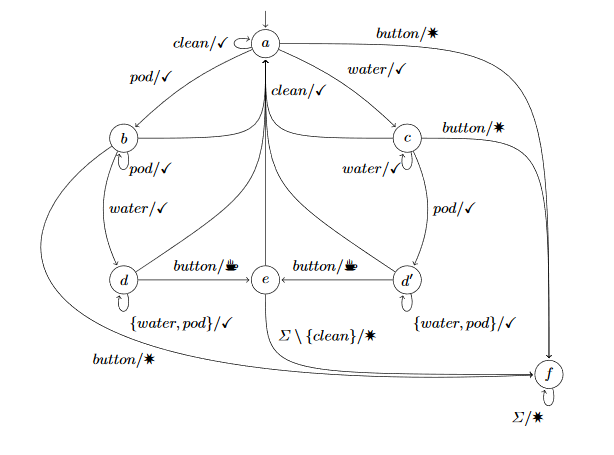
\includegraphics[width=0.7\linewidth]{content/coffeemealy}
	\caption{Mealy machine representing the functionality of a coffee machine.\cite{Steffen2011}}
	\label{fig:coffeemealy}
\end{figure}

Since automaton-based formalisms deal with alphabets, formal language theory is essential not only to define them, but to construct them in a way that is efficient in practical applications. Often automata are used to design and analyze real-life systems. Naturally, questions of efficiency and correctness arise, which is why the relations of automatons and formal languages are discussed more in-depth in the following subsection.

\subsection{Relations of formal languages and automata}

\begin{definition}[Recognized language of automata]
	The language $L\subseteq\Sigma$ containing all the accepted words by an automaton M is called the recognized language of the automaton. It is denoted by L(M) = L.
\end{definition}

\begin{definition}[Regular language]
	A formal language L is regular, iff there is a Deterministic Finite Automaton M, for which L(M) = L, in other words, iff there is a DFA with the recognized language of L.
\end{definition}

Let us now introduce a semantic helper $\delta^*$ for both DFAs and Mealy machines. $\delta^*$ is an extension of the $\delta$ transition function, as $\delta^*: S\times\Sigma^* \to S$ defined by $\delta^*(s,\epsilon) = s$ and $\delta^*(s, \alpha w) = \delta^*(\delta(s, \alpha), w)$, essentially providing the state of the automaton after running an input sequence from a specified state.

\begin{definition}[Myhill-Nerode relation] 
	A DFA $M=(S,s_{0},\Sigma,\delta,F)$ induces the following equivalence relation $\equiv_M$ on $\Sigma^*$ (when L(M) = $\Sigma$):\\
	\null\qquad$x\equiv_M y \iff \delta^*(s, x) = \delta^*(s, y)$\\
	where $x, y\in\Sigma^*$. This means, that x and y are equivalent with respect to $\equiv_M$.\cite{Kozen1977}.
\end{definition}

In words, the Myhill-Nerode relation states, that two words are equivalent wrt. $\equiv_M$ iff runs of both words would end in the same state on the automaton M. The Myhill-Nerode relation is an equivalence relation with some additional properties\cite{Kozen1977}, which can be seen in the following.


\begin{itemize}
	\item The properties of equivalence relations:
	\begin{itemize}
		\item Reflexivity: $x\equiv_M x$.
		\item Symmetry: $x\equiv_M y \implies y\equiv_M x$.
		\item Transitivity: if $(x\equiv_M y$ and $y\equiv_M z) \implies x\equiv_M z$.
	\end{itemize}
	\item Right congruence: $\forall x, y\in\Sigma^*: (x\equiv_M y \implies 		\forall a\in\Sigma: xa\equiv_Mya)$\\ also, by induction, this can be extended to:\\
	$\forall x, y\in\Sigma^*: (x\equiv_M y \implies \forall w\in\Sigma^*: xw\equiv_Myw)$. 
	\item It respects membership wrt. R:\\
	$\forall x, y\in\Sigma^*: x\equiv_M y \implies (x\in R \iff y\in R)$.
	\item $\equiv_M$ is of finite index, has finitely many equivalency classes. Since for every state $s\in S$, the sequences which end up in s are in the same equivalence class, the number of these classes is exactly $|S|$, which is a finite set.
\end{itemize}

Using this relation, we can introduce the Myhill-Nerode theorem, which neatly ties together the previous definitions.

\begin{theorem}[Myhill-Nerode theorem\cite{Kozen1977}\cite{10.2307/2033204}]
	Let $L\subseteq\Sigma^*$. The following three statements are equivalent:
	\begin{itemize}
		\item L is regular.
		\item there exists a Myhill-Nerode relation for L.
		\item the relation $\equiv_L$ is of finite index.
	\end{itemize}
	For proof, see \cite{Kozen1977}\cite{10.2307/2033204}.
\end{theorem}

The same concepts can be applied to Mealy machines, which are somewhat more complex in this regard. As before, a semantic helper is needed similar to $\delta^*$, but considering the output function of Mealy machines. $\lambda^*: S\times\Sigma^* \to \Omega$, defined by $\lambda^*(s, \epsilon) = \varnothing$ and $\lambda^*(s, w\alpha) = \lambda(\delta^*(s, w), \alpha)$.



When monitoring the behavior of Mealy machines, one of the most important metrics given an input is the specific output given by the input. The behavior of a Mealy machine, a specific run of it, has a pattern of \textit{$i_1,o_1,i_2,o_2,..,i_n,o_n$}, where \textit{i} are inputs and \textit{o} are outputs. In order to characterize these runs, we actually do not need every output from this pattern, we only need the final one. Also note, that essentially the final output of a run is given by $\lambda^*(s_0, inputs)$. Let us introduce a $\llbracket M\rrbracket$: $\Sigma^*\to\Omega$ semantic functional as  $\llbracket M\rrbracket(w) = \lambda^*(s_0, w)$. This provides the final output given by a run of an automaton for an input sequence $w$. Using $\llbracket M\rrbracket$, the behavior of Mealy machines can be captured, as discussed in the following.

\begin{example}
	Given the Mealy machine $M\textsubscript{coffeemachine}$ in Fig. \ref{fig:coffeemealy}, the runs:\\
	\null\qquad<clean, $\checkmark$>, \\
	\null\qquad<pod water button, \Coffeecup> \\
	are in $\llbracket M\textsubscript{coffeemachine}\rrbracket$, since the given input words cause the corresponding outputs, while the runs\\
	\null\qquad<clean, \Coffeecup> and \\
	\null\qquad<water button button, $\checkmark$> \\
	are not, since these input sequences do not produce those outputs.
\end{example}

Similarly to the Myhill-Nerode relations in DFAs, equivalence relations over the $P: \Sigma^*\to\Omega$ functional can be introduced, where P is an abstraction of  $\llbracket M\rrbracket$ that can be applied to any state, rather than just the initial state.

\begin{definition}[Equivalence of words wrt. $\equiv_P$\cite{Steffen2011}]
	Given a Mealy machine $M=(S,s_{0},\Sigma,\Omega,\delta,\lambda) $, two words, $u, u'\in\Sigma^*$ are equivalent with respect to $\equiv_P$:\\
	$u \equiv_P u' \iff (\forall v\in\Sigma^*:P(s, uv) = P(s, u'v))$.\\
	We write [u] to denote the equivalence class of u wrt. $\equiv_P$.
\end{definition}

This definition is more along the lines of the right congruence property observed in the Myhill-Nerode relations. The original formalism: $u \equiv_P u' \iff P(s, u) = P(s, u')$ of the Myhill-Nerode relation still stands as a special case of the above definition: if $v=\epsilon$ and $v'=\epsilon$, $P(s, uv) = P(s, u)$ and $P(s, u'v) = P(s, u')$.

\begin{example}
	Taking Fig. \ref{fig:coffeemealy} as an example, the following words are equivalent wrt. $\equiv_{\llbracket M\rrbracket}$:\\
	\null\qquad\qquad\qquad\qquad\space $water, pod$\\
	\null\qquad\qquad$\equiv_{\llbracket M\rrbracket}$\qquad $water, water, pod$\\
	\null\qquad\qquad$\equiv_{\llbracket M\rrbracket}$\qquad $pod, pod, water$.
	
	The first two of $\equiv_{\llbracket M\rrbracket}$ are straightforward, since both words lead to the same state, $d'$, while the third input ends in state $d$. Observably, state $d$ and $d'$ wrt. outputs operate exactly the same regardless of continuation, hence the equivalence holds.
\end{example}

\begin{theorem}[Characterization theorem\cite{Steffen2011}]
	Iff mapping $P: \Sigma^*\to\Omega$ $\equiv_P$ has finitely many equivalence classes, there exists a Mealy machine M, for which P is a semantic functional.
	\\\\
	\textit{Proof}($\impliedby$): As seen in the case of the Myhill-Nerode finite index property for DFAs, same states in Mealy machines will obviously be in same equivalence classes. This implies, that the number of classes in (or in other words, the index of) $\equiv_P$ is at most the number of states the Mealy machine contains, which is finite by definition.
	\\
	\textit{Proof}($\implies$): Consider the following Mealy machine: $M_P=(S,s_{0},\Sigma,\Omega,\delta,\lambda)$:\\
	\null\qquad -S is given by the equivalence classes of $\equiv_P$.\\
	\null\qquad -$s_0$ is given by $[\epsilon]$.\\
	\null\qquad -$\delta$ is defined by $\delta([u], \alpha) = [u\alpha]$.\\
	\null\qquad -$\lambda$ is defined by $\lambda([u], \alpha) = o$, where $P(u\alpha) = o$.\\
	A Mealy machine constructed this way fulfills what the theorem states, P is a semantic functional of it, in other words, $\llbracket M\rrbracket$ = P.
\end{theorem}

With this theorem, regularity for mappings $P:\Sigma^*\to\Omega$ can be defined. A $P:\Sigma^*\to\Omega$ mapping is regular, iff there is a corresponding Mealy machine for which $\llbracket M\rrbracket$ = P, or equivalently, if P has a finite number of equivalence classes, analogously to the previously seen "classical" regularity.

\subsection{Minimization of automata}

The introduction of regularity is useful in the construction of automata, specifically, the construction of canonical automata. 


\begin{figure}
	\centering
	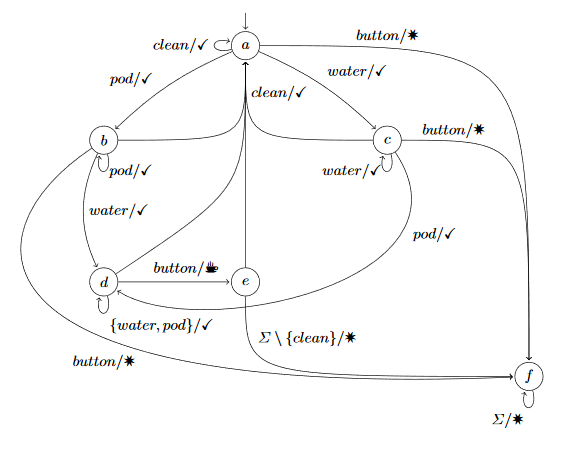
\includegraphics[width=0.7\linewidth]{include/coffeemealyminimal}
	\caption{Minimal version of the Mealy machine seen in \ref{fig:coffeemealy}}
	\label{fig:coffeemealyminimal}
\end{figure}


\begin{definition}[Canonical automaton (Minimal automaton)]
	An automaton M is canonical (i.e. minimal) iff:
	\begin{itemize}
		\item every state is reachable: $\forall s\in S: \exists w\in\Sigma^*: \delta^*(s_0, w) = s$,
		\item all states are pairwisely separable, in other words behaviorally distinguishable. For Mealy machines, this is formalized as: $\forall s_1, s_2\in S: \exists w\in\Sigma^*: \lambda(s_1, w)\neq\lambda(s_2, w)$
	\end{itemize}
\end{definition}

The minimal version of the Mealy machine in Fig. \ref{fig:coffeemealy} can be seen in Fig. \ref{fig:coffeemealyminimal}.


Constructing automata to be canonical, especially in the case of Mealy machines is important with regards to efficiency and is the backbone of automaton learning. The next proposition comes straightforward from the previously presented characterization theorem.


\noindent \textbf{Proposition (Bounded reachability\cite{Steffen2011})}: Every state of a minimal Mealy machine with n states has an access sequence, i.e., a path from the initial state to the given state,  of  length  at  most n-1.  Every  transition  of the model can be covered by a sequence of length at most n from the initial state.

The process of constructing automata uses the concept of partition refinement. It works based on distinguishing suffixes, suffixes of words which mark, witness the difference between two access sequences. The following notion is introduced to formalize this.


\begin{definition}[k-distinguishability\cite{Steffen2011}]
	Two states, $s,s'\in S$ are k-distinguishable iff there is a word $w\in\Sigma^*$ of length k or shorter, for which $\lambda^*(s, w)\neq\lambda^*(s',w)$.
\end{definition} 

\begin{definition}[exact k-distinguishability]
	Two states, $s,s'\in S$ are exact k-distinguishable, denoted by $k^=$ iff s and s' are k-distinguishable, but not (k-1)-distinguishable
\end{definition}

Essentially, if two states, s and s' are  k-distinguishable, then when processing the same input sequence, from some suffix of the word w with length at most k, they will produce differing outputs. Using this, we can observe, that whenever two states, $s_1, s_2\in S$ are (k+1)-distinguishable, then they each have a successor $s_1'$ and $s_2'$ reached by some $\alpha\in\Sigma$, such that $s_1'$ and $s_2'$ are k-distinguishable. These successors are called $\alpha$-successors. This suggests, that:
\begin{itemize}
	\item no states are 0-distinguishable and
	\item two states $s_1$ and s2 are (k+1)-distinguishable iff there exists an input symbol $\alpha\in\Sigma$, such that $\lambda(s_1, \alpha) \neq \lambda(s_2,\alpha)$ or $\delta(s_1, \alpha)$ and $\delta(s_2, \alpha)$ are k-distinguishable.\cite{Steffen2011}
\end{itemize}
This way, if we have an automaton M, we can construct its minimal version, by iteratively computing k-distinguishability for increasing k, until stability, that is until the set of exactly k-distinguishable states is empty.

\begin{example}
	Given the Mealy machine seen in Fig.\ref{fig:coffeemealy}, we can use k-distinguishability to refine its partitions. The initial state, the initial partition would be:\\
	$P_1 = \{a, b, c\}, \{d, d'\}, \{e\}, \{f\}$\\
	since when k=1, a, b and c are not 1-distinguishable, but d and d' separate on the behavior of the \textit{button} input, while e and f are separated by the suffix \textit{clean}. Let's see the k=2 scenario.\\
	$P_2 = \{a\}, \{b\}, \{c\}, \{d, d'\}, \{e\}, \{f\}$\\
	Here, \textit{water} and \textit{pod} separate a, b and c, while d and d' can still no longer be separated. If observed, even if k is increased, d and d' can not be refined. This means, that they are indistinguishable, they can be merged together without altering behavior. This shows the process of acquiring the minimal machine seen in Fig. \ref{fig:coffeemealyminimal}.
	\label{ex:partitionrefinement}
\end{example} 

The process explained in Example \ref{ex:partitionrefinement} is partition refinement, the exact algorithm and proof of its validity can be seen in \cite{Steffen2011}. Partition refinement is a version of the minimization algorithm for DFAs proposed by Hopcroft\cite{HOPCROFT1971189}. 

Let us define one last relation which will be useful in the next section to compare automata minimization and automata learning.

\begin{definition}[k-epimorphisms]
	Let $M=(S,s_{0},\Sigma,\Omega,\delta,\lambda)$ and $M=(S',s_{0}',\Sigma,\Omega,\delta',\lambda')$ be two Mealy machines with shared alphabets. We call a surjective function $f_k: S \to S'$ existential k-epimorphism between $M$ and $M'$, if for all $s'\in S', s\in S$ where $f_k(s) = s'$ and with any $\alpha\in\Sigma$, we have: $f_k(\delta(s,\alpha)) = \delta'(s',\alpha)$, and all states, that are mapped by $f_k$ to the same state of $M'$ are not k-distinguishable.
\end{definition}

 It is straightforward to establish that all intermediate models arising during the partition refinement process are images of the considered Mealy machine under a k-epimorphism, where k is the number of times all transitions have been investigated.\cite{Steffen2011} Essentially this establishes $P_1$ and $P_2$ from Example \ref*{ex:partitionrefinement} as images of the Mealy machine seen in Fig. \ref{ex:coffeemealy} under k-epimorphisms where k=1 and k=2 respectively.

Active automaton learning algorithms operate in a similar way, but they do not have access to the automata they are learning.



\section{Automaton learning}



\paragraph{Automaton learning}  is a way of modeling a system without having specific knowledge of its internal behavior. To accomplish this, the external behavior of the system needs to be observed. This learned model is, as the name suggests, an automaton. 
\\Formally: Automata  learning is  concerned  with  the  problem  of  inferring  an automaton model for an unknown formal language $L$ over some alphabet $\Sigma$\cite{Howar2018}.
\\\\In order to monitor a system, access to its behavioral information is required. There are two approaches, which separate the two types of automaton learning.

\paragraph{Passive automaton learning} In case of passive automaton learning, the gathering of information is not part of the learning process, but rather a prerequisite to it. The learning is performed on a pre-gathered positive an/or negative example set of the systems behavior. In passive automaton learning, the success of the process is determined not only by the efficiency of the algorithm, but the methodology and time used to gather the data.

\paragraph{Active automaton learning} In case of active automaton learning, the behavioral infromation is gathered by the learning algorithm via queries. In order to accomplish this, learning is separated to two components: the learner, which learns, and the teacher, which can answer questions about the system under learning.


Active automaton learning follows the MAT, or the Minimally Adequate Teacher model proposed by Dana Angluin\cite{ANGLUIN198787}. It defines the separation of the algorithm to a teacher and a learner component in a way, where the teacher can only answer the minimally adequate questions needed to learn the system. These two questions, or queries are are follows:


\paragraph{Membership query} Given a $w\in\Sigma^{*}$ word, the query return the $o\in \Omega$ output o corresponding to it, treating the word as a string of inputs. We write $mq(w) = o$ to denote that executing the query w on the system under learning (SUL) leads to the output o: $\llbracket SUL \rrbracket(w) = o$ or $\lambda^*(s_0, w) = o$.

\paragraph{Equivalence query} Given a hypothesis automaton $M$, the query attempts to determine if the hypothesis is behaviorally equivalent to the SUL, and if not, finding the diverging behavior, and return with an example. We write $eq(H) = c$, where $c\in\Sigma^*$, to denote an equivalence query on hypothesis H, returning a counterexample c. The counter example provided is the sequence of inputs for which the output of system under learning and the output of the hypothesis differ: $ \llbracket H\rrbracket(c) \neq mq(c)$.

\noindent The learner component uses membership queries to construct a hypothesis automaton, then refines this hypothesis by the counterexamples provided by equivalence queries. Once counterexamples can not be found this way, the learners hypothesis is behaviorally equivalent to the SUL. The learning can terminate and the output of the learning is the current hypothesis.

\begin{figure}[H]
	\centering
	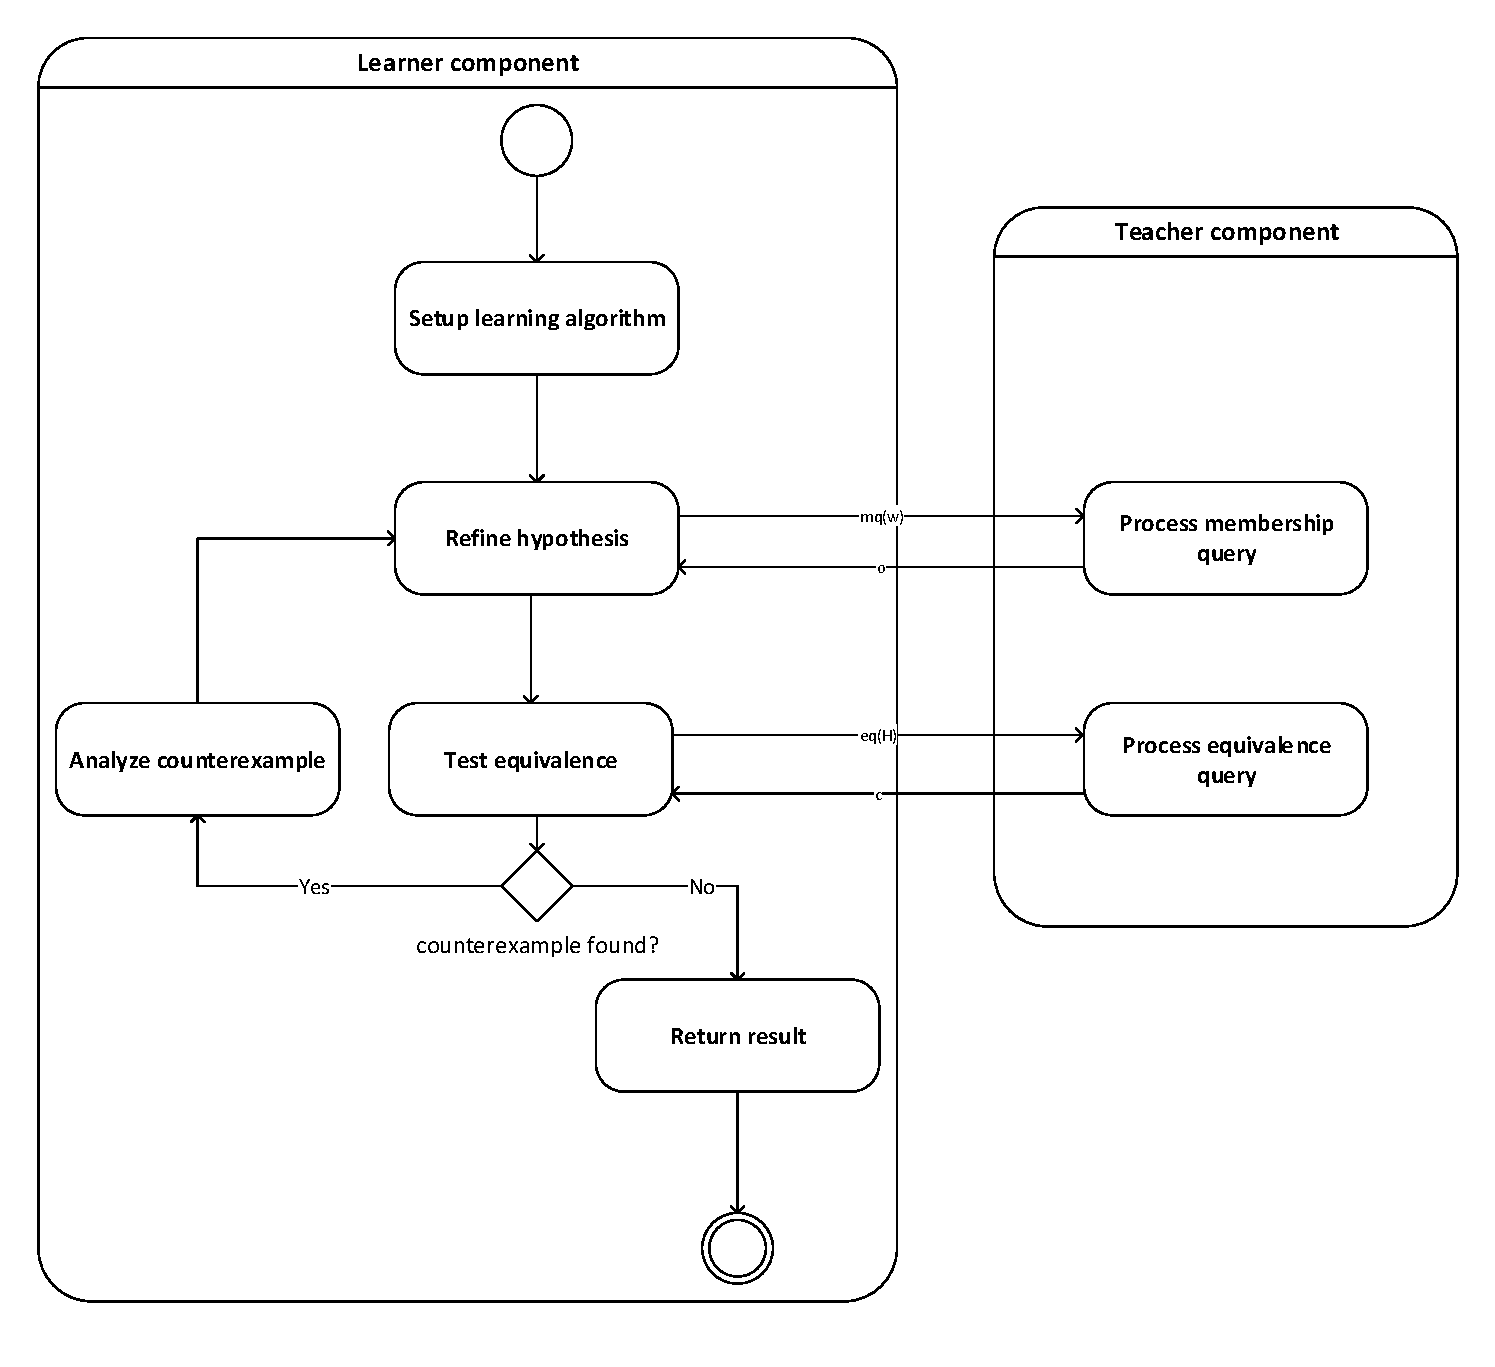
\includegraphics[width=1.0\linewidth]{figures/flowchartlearning}
	\caption{Active automaton learning}
	\label{fig:flowchartlearning}
\end{figure}

As seen on Fig. \ref{fig:flowchartlearning}, the learning proceeds in rounds, generating and refining hypothesis models by exploring the SUL via membership queries. As the equivalence checks produce counterexamples, the next round of this hypothesis refinement is driven by the counterexamples produced.

Using an analogous strategy to the minimization of automata seen in the previous section, starting only with a one state hypothesis automaton, all words are explored in the alphabet in order to refine and extend this hypothesis. Here, there is a dual way of characterizing (and distinguishing) between states\cite{Steffen2011}:
\begin{itemize}
	\item By words reaching them. A prefix-closed set $S_p$ of words, reaching each state exactly once, defines a spanning tree of the automaton. This characterization aims at providing exactly one representative element from each class of $\equiv_P$ on the SUL. Active learning algorithms incrementally construct such a set $S_p$. \\This prefix-closedness is necessary for $S_p$ to be a "spanning tree" of the Mealy machine. Extending $S_p$ with all the one-letter continuations of words in $S_p$ will result in the tree covering all the transitions of the Mealy machine. $L_p$ will denote all the one-letter continuations that are not already contained in $S_p$.
	\item By their future behavior with respect to an increasing vector of words of $\Sigma^*$. This vector $<d_1, d_2,...,d_k>$ will be denoted by $D$, and contains the "distinguishing suffixes". The corresponding future behavior of a state, here given in terms of its access sequence $u\in S_p$, is the output vector$<mq(u*d_1), ..., mq(u*d_k)>\in\Omega^k$, which leads to an upper approximation of the classes of $\equiv_{\llbracket SUL\rrbracket}$. Active learning incrementally refines this approximation by extending the vector until the approximation is precise.
\end{itemize}
While the second characterization defines the states of the automaton, where each output vector corresponds to one state, the spanning tree on $L_p$ is used to determine the transitions of these states. In order to characterize the relation between the SUL $M=(S,s_{0},\Sigma,\Omega,\delta,\lambda)$ and the hypothesis model $M'=(S',s_{0}',\Sigma,\Omega,\delta',\lambda')$ (note, that $M$ and $M'$ only share alphabets), the following definition is introduced. 

\begin{definition}[D-epimorphism]
	Let $D\subseteq\Sigma^*$. We call a surjective function $f_D:S\to S'$ existential D-epimorphism (surjective homomorphism) between $M$ and $M'$ if, for all $s'\in S'$ there exists an $s\in S$ with $f_D(s) = s'$ such that for all $\alpha \in \Sigma$ and all $d\in D$: $f_D(\delta(s, \alpha)) = \delta'(s', \alpha)$, and $\lambda^*(s,d) = \lambda^*(s', d)$. 
\end{definition}

Note, that active learning deals with canonical Mealy machines, in other words, the canonical form of SUL, and not, the perhaps much larger Mealy machine of SUL itself. 

Since active learning algorithms maintain an incrementally growing extended spanning tree for $H=(S_H, h_0, \Sigma, \Omega, \delta_H, \lambda_H)$, i.e., a prefix-closed set of words reaching all its states and covering all transitions, it is straightforward to establish that these hypothesis models are images of the canonical version of SUL under a canonical existential D-epimorphism, where D is the set of distinctive futures underlying the hypothesis construction\cite{Steffen2011}
\begin{itemize}
	\item define $f_D : S_{SUL}\to S_H$ by $f_D(s) = h$ as following: if $\exists w\in S_p \cup L_p$, where $\delta(s_0, w) = s$, then $h = \delta_H(h_0,w)$. Otherwise h may be chosen arbitrarily.
	\item It suffices to consider the states reached by words in the spanning tree to establish the defining properties of $f_D$. This straightforwardly yields:
	\begin{itemize}
		\item $f_D(\delta(s,\alpha)) = \delta_H(h, \alpha)$ for all $\alpha\in\Sigma$, which reflects the characterization from below.
		\item $\lambda^*(s, d) = \lambda^*_H(h,d)$ for all $d\in D$, which follows from the maintained characterization from above.\cite{Steffen2011}
	\end{itemize}
\end{itemize}

In basic logic, D-epimorphisms and k-epimorphisms do not differ, they both deal with establishing constructed models being images of the model they are based on. D-epimorphisms could replace k-epimorphisms where $D=\Sigma^k$, it can be suggested, that there is no need to differentiate. However, there is in important difference of complexity between the two. While k-distinguishability supports polynomial time, black-box systems do not. Also, the "existential" in existential D-epimorphism is important: $f_D$ must deal with unknown states, ones that haven't been encountered yet. This implies that characterization can only be valid for already encountered states.

Active learning algorithms can be proven correct using the following three-step pattern:
\begin{itemize}
	\item Invariance: The number of states of each hypothesis has an upper bound of $\equiv_{\llbracket SUL\rrbracket}$.
	\item Progress: Before the final partition is reached, an equivalence query will provide a counterexample, where an input word leads to a different output on the SUL and on the hypothesis. This difference can only be resolved by splitting at least one state, which increases the state count.
	\item Termination: The refinement terminates after at most the index of $\equiv_{\llbracket SUL\rrbracket}$ many steps, caused directly by the described invariance and progress properties.
\end{itemize}

The following subsection introduces the first active automaton learning algorithm this thesis covers.

\subsection{Direct Hypothesis Construction\cite{10.1007/978-3-642-34781-8_19}}
The Direct Hypothesis Construction algorithm, which hypothesis construction can be seen in Algorithm \ref{algo:dhc}  follows the idea of the breath-first search of graph theory. It constructs the hypothesis using a queue of states, which is initialized with the states of the spanning tree to be maintained. Explored states are removed from this queue, while the discovered successors are enqueued, if they are provably new states. The algorithm starts with a one-state hypothesis, including only the initial state, reached by $\epsilon$ and D = $\Sigma$. It then tries to complete the hypothesis: for every state, the algorithm determines the behavior of the state under D. This behavior is called the extended signature of said state. States with a new extended signatures are provably new states, so to guarantee further investigation, all their successors are enqueued. Initially, $D=\Sigma$, so only the $1^=$-distinguishable states are revealed during the first iteration. This is extended straightforwardly to comprise a prefix closed set of access sequences. \cite{Steffen2011}\cite{10.1007/978-3-642-34781-8_19}

\begin{algorithm}[H]
	\SetAlgoLined
	\DontPrintSemicolon
	\KwIn{$S_p$: a set of access sequences, D: a set of suffixes, an input alphabet $\Sigma$}
	\KwOut{A Mealy machine $H=(S, s_0, \Sigma, \Omega, \delta, \lambda)$}
	initialize hypothesis H, create a state for all elements of $S_p$\;
	initialize a queue Q with the states of H\;
	\While{Q is not empty}{
		s = dequeue state from Q\;
		u = access sequence from $s_0$ to s\;
		\For{$d\in D$}{
			o = mq($u\*d$)\;
			set $\lambda(s,d) = o$\;
		}
		\eIf{exists an $s'\in S$, where the output signature of $s'$ is the same as $s$}{
			reroute transitions of $s$ to $s'$ in H\;
			remove $s$ from H\;
		}{
			create and enqueue successors of $s$ for every input in $\Sigma$ into Q, if not already in $S_p$\;
		}
	}
	Remove entries of $D\setminus\Sigma$ from $\lambda$\;
	\Return{H}\;
	\caption{Hypothesis construction of the Direct Hypothesis Construction algorithm as seen in \cite{Steffen2011}.}
	\label{algo:dhc}
\end{algorithm}

After the execution of the Hypothesis construction seen in Algorithm \ref{algo:dhc}, the output automaton H is used in an equivalence query $eq(H) = c$, to find if a counterexample $c$ exists. If no counteraxamle can be found, the learning terminates, $H$ is the learned automaton. Else, if a counterexample $c$ is found, for which $\lambda_H(s_0,c) \neq mq(c)$, $c$ is used to enlarge the suffixes in D and a new iteration of Algorithm \ref{algo:dhc} begins, using the now extended set D and all the access sequences found in the previous iteration (the current spanning tree $S_p$).

While the DHC algorithm is a straightforward implementation of active automata learning, it struggles with time complexity. It terminates after at most $n^3mk+n^2k^2$ membership queries, and $n$ equivalence queries, where $n$ is the number of states in the final hypothesis, $k$ is the longest set of inputs, and $m$ is the length of the longest counterexample. This renders the DHC algorithm inefficient in practical applications. The next subsection deals with an optimized algorithm, the TTT algorithm.

\subsection{The TTT algorithm\cite{10.1007/978-3-319-11164-3_26}}

As seen in the Direct Hypothesis Construction algorithm, a large number membership queries are required in order to learn an automaton, causing a bottleneck on the scalability of the algorithm. The main cause of this complexity issue is the way counterexamples are treated. In order to ensure every state is properly found, \textit{all} suffixes of the counterexample are added to the algorithms structure, which, has a huge impact on the number of membership queries in the next iteration of the hypothesis construction. TTT resolves this inefficiency by fine-tuning exactly what needs to be further investigated by membership queries.\\

\begin{example}
	As an example, we'll use the automaton portrayed on Fig.\ref{fig:dfaexamplemealyver}.a, a Mealy machine version of the DFA previously seen in Fig.\ref{fig:dfaexample} constructed simply by the following rule: if a transition ends in $q_3$, the output is $\bot$, else the output is $\top$.
	\\TTT keeps the notion of separating states by a spanning tree $S_p$, a prefix-closed set of words from $\Sigma^*$, this tree defines the access sequences of each state. The spanning tree $S_p$ is indicated by bold transitions in Fig.\ref{fig:dfaexamplemealyver}.a. 
	\\States are separated by the notion of discriminators. The algorithm maintains a set of discriminator suffixes D, but uses them differently from the DHC algorithm. D in TTT is used by a n-ary tree, where n = $|\Omega|$, so in this example a binary tree. We call this tree a discrimination tree (seen in Fig.\ref{fig:dfaexamplemealyver}.b), which maintains information about which inputs (discriminators) separate states: for every distinct pair of states, a separator can be obtained by looking at the label of the lowest common ancestor of the corresponding leaves. This way, the label of inner nodes act as discriminators. These labels form a suffix-close set and are stored in a trie seen in Fig.\ref{fig:dfaexamplemealyver}.c. Each node of the trie is a word, which can be constructed by going up the tree towards the root.
\end{example}

\begin{figure}[H]
	\centering
	\begin{subfigure}{0.35\textwidth}
		\centering
		\begin{tikzpicture}[shorten >=1pt,node distance=3.5cm,on grid,auto] 
		\node[state,initial] (q_0)   {$q_0$}; 
		\node[state] (q_1) [right=of q_0] {$q_1$}; 
		\node[state] (q_2) [below=of q_0] {$q_2$}; 
		\node[state](q_3) [right=of q_2] {$q_3$};
		\path[->] 
		(q_0) edge[line width = 0.4mm]  node {a/$\top$} (q_1)
		edge [loop below] node {b/$\top$} ()
		(q_1) edge[line width = 0.4mm]  node[pos=0.62]  {a/$\top$} (q_2)
		edge [loop below] node {b/$\top$} ()
		(q_2) edge[line width = 0.4mm]  node [swap] {a/$\bot$} (q_3) 
		edge [loop above] node {b/$\top$} ()
		(q_3) edge  node[pos=0.62] [swap] {a/$\top$} (q_0)
		edge [loop above] node {b/$\bot$} () ;
		\end{tikzpicture}
		\caption{A Mealy-machine version of the DFA seen in Fig. \ref{fig:dfaexample}.}
	\end{subfigure}
	\begin{subfigure}{0.55\textwidth}
		\centering
		\begin{tikzpicture}[shorten >=1pt,node distance=1.8cm,on grid,auto] 
		\node[state] (e)   {$\epsilon$}; 
		\node[state] (a) [below left=of e] {$a$}; 
		\node[state] (q3) [right=of a] {$q_3$}; 
		\node[state] (aa) [below left=of a] {$aa$};
		\node[state] (q2) [right=of aa] {$q_2$}; 
		\node[state] (q0) [below left=of aa] {$q_0$}; 
		\node[state] (q1) [right=of q0] {$q_1$}; 
		\path[->] 
		(e) edge node {} (a)
		(e) edge node {} (q3)
		(a) edge node {} (aa)
		(a) edge node {} (q2)
		(aa) edge node {} (q0)
		(aa) edge node {} (q1);
		\end{tikzpicture}
		\caption{Final discrimination tree.}
	\end{subfigure}
	\begin{subfigure}{0.2\textwidth}
		\centering
		\begin{tikzpicture}[shorten >=1pt,node distance=1.8cm,on grid,auto] 
		\node[state] (e)   {$\epsilon$}; 
		\node[state] (a) [below=of e] {$a$}; 
		\node[state](aa) [below=of a] {$aa$};
		\path[->] 
		(aa) edge node {a} (a)
		(a) edge node {a} (e);
		\end{tikzpicture}
		\caption{Discriminator trie of the final hypothesis.}
	\end{subfigure}	
	\caption{The three namesake trees of the TTT algorithm, (a) being a spanning \textbf{T}ree, (b) a disctimination \textbf{T}ree, and (c) a discriminator \textbf{T}rie.}
	\label{fig:dfaexamplemealyver}
\end{figure}


Discriminator trees, as seen in the previous example, are rooted n-ary trees, where n is the size of the output alphabet. Leaves are labeled by states of the automaton, while inner states are labeled by discriminators (suffixes). When adding a new word to the tree $T$, we sift the word $w\in\Sigma^*$ into T by starting at the root, and for every inner node $v\in D$, we branch depending on the output of $\lambda^*(wu)$. This limits the number of membership queries to the height of the tree, while DHCs limit was $S_p\times D$.
\\\\
\textbf{Key steps of the TTT algorithm:}
\begin{itemize}
	\item \textbf{Hypothesis construction.} The initial state is initialized and membership queried for all inputs, the results of which are sifted into the discriminator tree T.
	\item \textbf{Hypothesis refinement.} If a counterexample is found, the corresponding state is split (analogously to the DHC algorithm), in the discriminator tree, the leaf corresponding to this new state is split by a temporary discriminator $v\in\Sigma$.
	\item \textbf{Hypothesis stabilization.} The hypothesis provided by the previous example might contradict information of the discrimination tree. This step searches for counterexamples between them (without the need of equivalence queries), and if any such counterexample exist, states are split accordingly.
	\item \textbf{Discriminator finalization.} TTT treats discriminators derived directly from counterexamples temporary, keeping track of the maximal sub-tree of the discrimination tree containing temporary discriminators. This sub-tree is split as temporary discriminators are replaced with final ones. Only when this finalization happens, is an inner node of the discrimination tree considered a member of the discriminator trie, in other words, when finalizing a temporary discriminator, it is added to the discriminator trie.
\end{itemize}
For a more detailed description of the TTT algorithm the reader is referred to\cite{10.1007/978-3-319-11164-3_26}.
\chapter{Contribution}\label{contrib}

The main contribution of this thesis is an active automaton learning framework, which can be used to support system design and analysis. This framework, since used in system engineering, is required to be easily modifiable and extensible, while having the capability of handling any variation of formalisms systems might rely on.


\section{Automaton learning framework}

Active automaton learning algorithms essentially have two endpoints: the input, reached through the teacher component, and the output, where the learned hypothesis automaton is returned. This is illustrated in Fig. \ref{fig:learningcomm}. The teacher and the learner can be adjusted to the required formalisms: the underlying modeling language of the system under learning (the \emph{input formalism}) and that of the learned hypothesis (the \emph{output formalism}). \\
\begin{figure}[H]
	\centering
	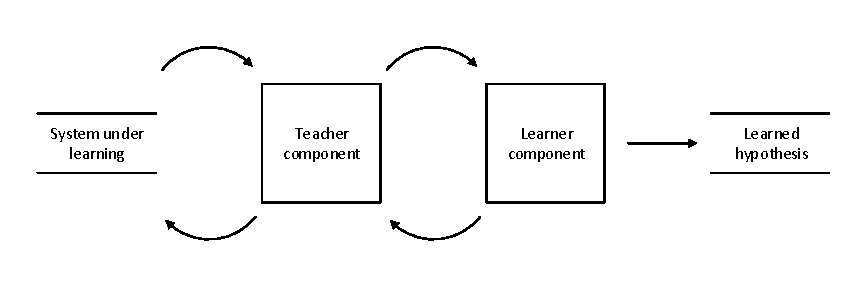
\includegraphics[width=1.0\linewidth]{figures/learningcomm}
	\caption{Data flow of active learning algorithms.}
	\label{fig:learningcomm}
\end{figure}

\subsection{Tooling}

As seen in Fig. \ref{fig:learningcomm}, the variables of the framework are essentially the input and output formalisms it accepts. Tooling was used to both ensure flexibility in this regard and as way to provide future integration. Specifically, the \emph{Gamma Statechart Composition framework}\cite{DBLP:conf/icse/MolnarGVMV18} and the \emph{Theta framework}\cite{theta-fmcad2017} enable the use of the learned automaton in furthering the design of a system (component). Since both Gamma and Theta are implemented in Java/\emph{EMF}, and \emph{Xtext} has native integration with \emph{EMF}, these two tools were used, and are described in the following.

\begin{itemize}
	\item \textbf{Eclipse Modeling Framework (EMF):} EMF, or more specifically, EMF core, is an "abstraction for describing, composing, and manipulating structured information", essentially a tool for system modeling and code generation implemented in Java. The tool it provides allows graphical modeling of UML class diagrams and generating code based on these models.
	\item \textbf{Xtext:} Xtext is a framework for creating programming and domain-specific languages, which also has integration with EMF. This integration allows reading and writing text files in the form of an Xtext grammar using corresponding EMF generated classes.
\end{itemize}


\subsection{High-level overview}

Since the implementation of the framework would be using Java as a language, the high-level view seen in Fig. \ref{fig:abstractoverview} is an UML class diagram of the packages and the relations between them, essentially being an overview of the modularization of the framework.

\begin{figure}[H]
	\centering
	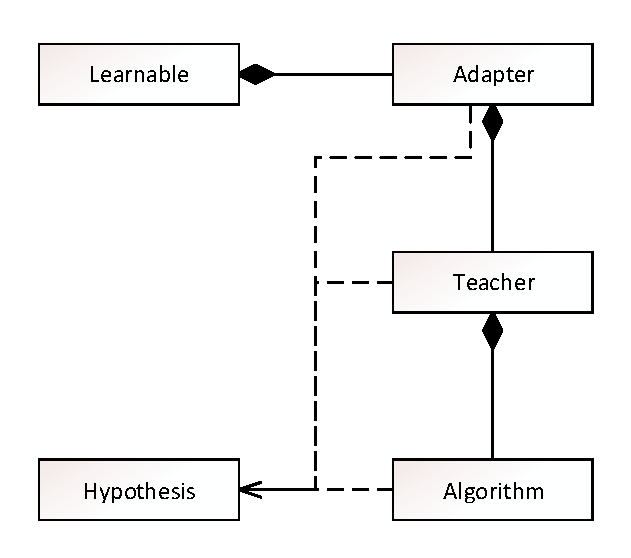
\includegraphics[width=0.5\linewidth]{figures/abstractoverview}
	\caption{Structure and relations of the packages comprising the framework.}
	\label{fig:abstractoverview}
\end{figure}

Note, that when comparing Fig. \ref{fig:abstractoverview} to Fig. \ref{fig:learningcomm}, the data flows identically. The \emph{Learnable} package containing the input formalisms, and the Hypothesis package containing the output formalisms are used by the teacher (\emph{Teacher} package) and the learner (\emph{Algorithm} package). The package not represented on Fig. \ref{fig:learningcomm}, the \emph{Adapter} package is used as an abstraction layer to separate the algorithm and the teacher from the input formalism. Since automaton learning algorithms have no direct access to the system under learning, they operate in a black-box way, the \emph{Adapter} package is a useful addition. Unfortunately no such adapter can be used on the output layer, since Hypotheses are directly accessed by the learning algorithms, and are constructed during the learning. While more specific abstractions were made (and can be seen later), no singular abstraction layer can be provided for every type of automaton and every type of learning algorithm the same way as for the input formalisms.
\\\\
The relations between the packages (modules) are straightforward. Composition is used, to indicate, that there is no \emph{Algorithm} (learner) without a \emph{Teacher}, there is no \emph{Teacher} without an \emph{Adapter}, and there is no \emph{Adapter} without an input, a \emph{Learnable}, to adapt. \emph{Algorithm}s of course depend on \emph{Hypothesis}, and because of equivalence queries, which are later transferred through the Teacher and Adapter components, they both also have a dependency on the \emph{Hypothesis} package.

\subsection{Detailed overview of abstractions}


The diagram in Figure \ref{fig:abstractoverview} showed the modularization of the framework, which depend on the correct implementation of object-oriented architecture so the notated compositions and dependencies in Fig. \ref{fig:abstractoverview} are satisfied. These abstractions are defined and implemented in Java as abstract classes and interfaces seen in Fig. \ref{fig:abstractdetailedoverview}. The detailed descriptions of these abstractions are as follows.
\\
\begin{itemize}
	\item \textbf{Learnable:} The \emph{Learnable} interface is the input type used by the framework. It defines two generic parameters, \emph{I} is the character type of the regular language the Learnable represents, while \emph{O} is the character type by which actions are defined for the system under learning. The only method the interface defines is the \emph{getOutput()} method, which returns the output \emph{O} given by the system under learning for a specific sequence of inputs. Note, that while the word "output" is used, the \emph{O} it returns is the action the system takes for an input. If the system is represented as a DFA, this would be the state it moves to, if the system is represented as a Mealy machine, it would be an output.
	
	\item \textbf{Hypothesis:} The \emph{Hypothesis} interface is the output type used by the framework. The generic parameters it takes are the automaton it uses (\emph{M}), and the input (\emph{I}), output (\emph{O}), state (\emph{S}) and transition (\emph{T}) types used by \emph{M}. The Hypothesis interface does not enforce bounds on these parameters to allow flexibility in implementation. Beyond the getters, the \emph{query()} method takes a sequence of inputs, and returns the output given by the hypothesis automaton. Just as with the \emph{Learnable} interface, this output represents action in the automaton.
	
	\item \textbf{LearnableAdapter:} The \emph{LearnableAdapter} abstract class is the abstraction of the adaptation between any \emph{Learnables} and \emph{Hypotheses}. The generic parameters of it are the \emph{Hypothesis} type (\emph{H}) and the input, output types of \emph{H} (\emph{HI}, \emph{HO}), similarly, the \emph{Learnable} type (\emph{L}) and the input, output types of \emph{L} (\emph{LI}, \emph{LO}). The \emph{LearnableAdapter} class stores a \emph{Learnable}, the object which represents the data of the system under learning. It gives access to the system using the \emph{membershipQuery()} method and the abstract \emph{equivalenceQuery()} method. The abstract \emph{covert..()} methods are used to do the actual adapting between \emph{Hypotheses} and \emph{Learnables} character by character.
	
	\item \textbf{Teacher:} The \emph{Teacher} abstract class defines the "middle ground" between a learning algorithm and the input. The \emph{Teacher} class as generic parameter, takes a \emph{Hypothesis} (\emph{H}) with input and outputs types of \emph{HI} and \emph{HO}, also a \emph{LearnableAdapter} (\emph{LA}) which has the same \emph{Hypothesis} type as \emph{H}. It defines two query types, \emph{membershipQuery()} and \emph{equivalenceQuery}, both of which it delegates to the current adapter object in its adapter field. The \emph{Teacher class} is needed for easy extensibility, specifically, for any algorithm and input to work together without modification on them.
	
	\item \textbf{ActiveLearningAlgorithm:} The \emph{ActiveLearningAlgorithm} class provides abstraction for active automaton learning algorithms. It defines only a \emph{Hypothesis}  (\emph{H}), and its input types (\emph{HI}, \emph{HO}). The teacher field bounded to the \emph{Hypothesis} \emph{H} is used for queries, while the \emph{execute()} method executes the algorithm and returns with the learned \emph{Hypothesis}. Note, that the algorithm is fully separated from the system it is learning, it does not even know the generic type which with the communication, queries are executed.
\end{itemize}


\begin{figure}[H]
	\centering
	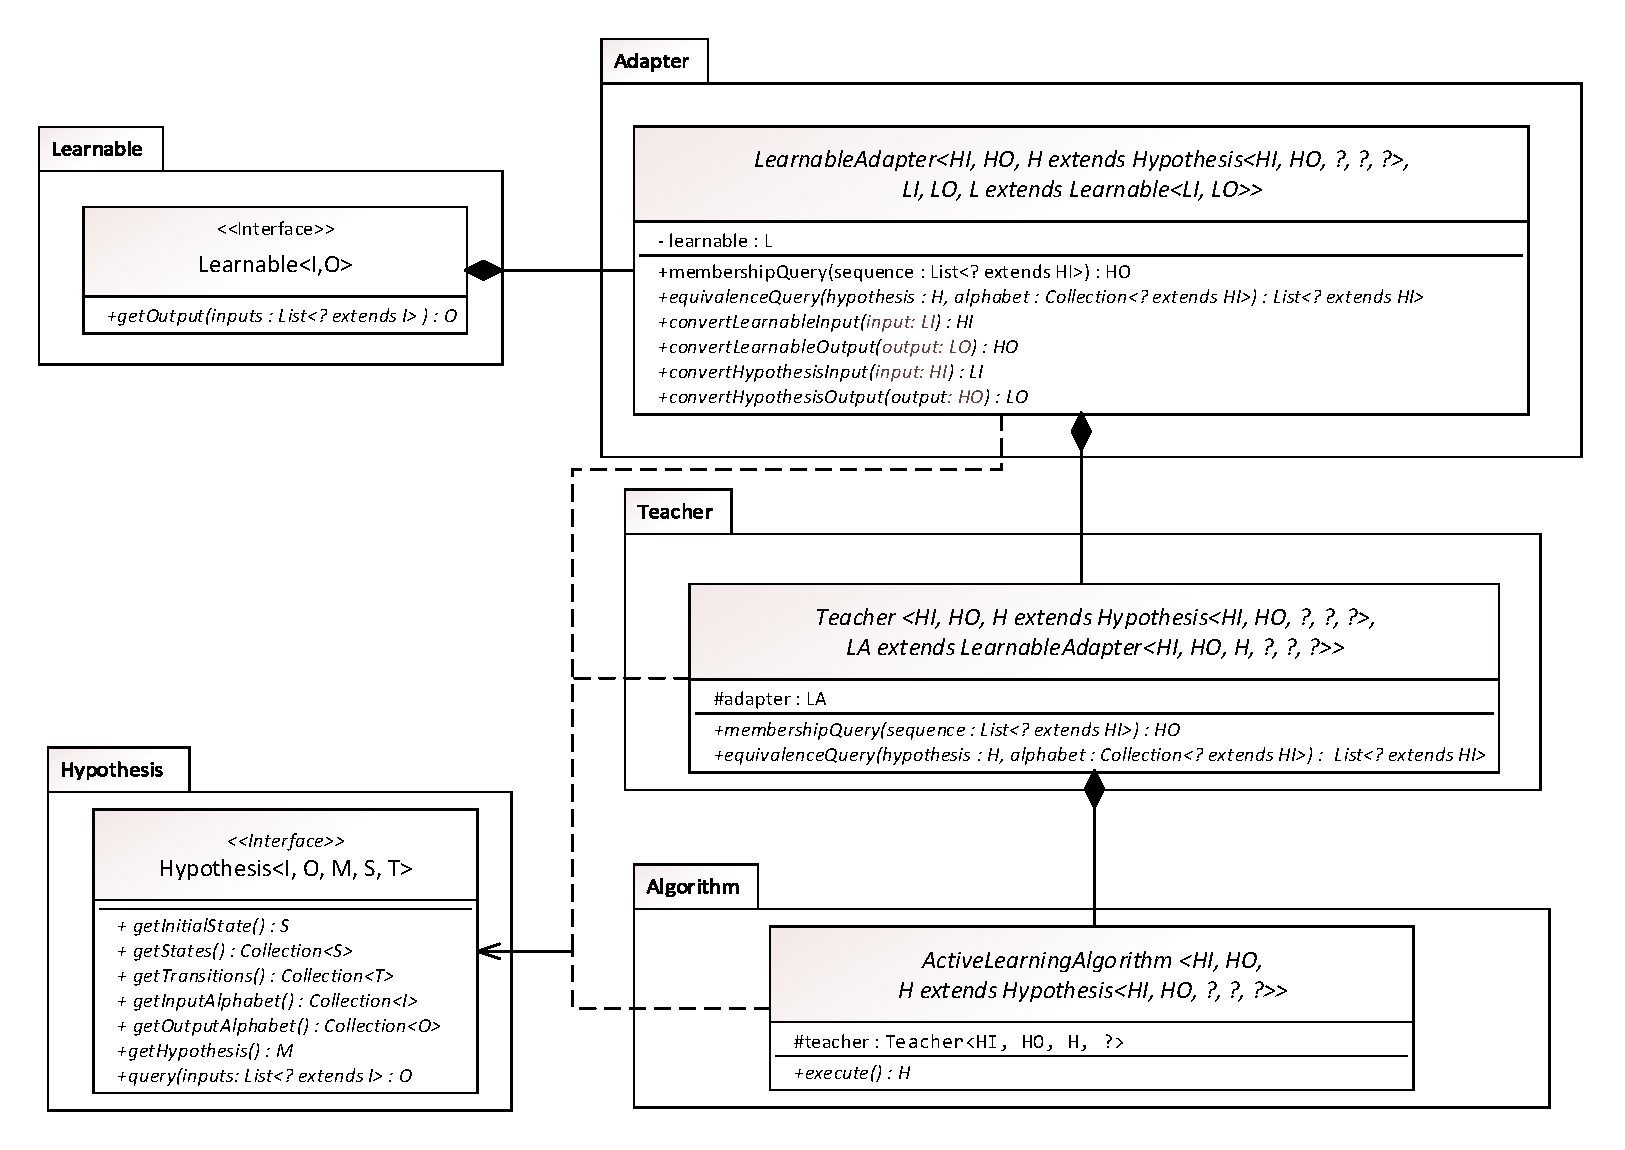
\includegraphics[width=0.97\linewidth]{figures/abstractdetailedoverview}
	\caption{Overview of the abstract classes and interfaces of the framework.}
	\label{fig:abstractdetailedoverview}
\end{figure}

\section{Implemented learning algorithms}

Building upon the abstractions of the framework, I implemented the two active learning algorithms presented in Chapter \ref{background}. The first step of the implementation was determining the input and output formalisms to use.

Since automaton learning algorithms can be implemented on any type of automata, the easiest method would be using deterministic finite automata. However, real-life reactive systems are usually better modeled using Mealy machines, hence the implementation was made using Mealy machines as both input and output formalisms.
\\
The first step of the implementation process was choosing the right tooling, which is why the Mealy machine implementation was done in Eclipse Modeling Framework.
\\\\
Figure \ref*{fig:mealyecore} shows an UML class diagram of the metamodel I've created using the Ecore package of EMF core, and the graphical modeling tool provided by EMF. I also used EMF to generate Java classes corresponding to the ones seen in Fig. \ref{fig:mealyecore}.

\begin{figure}
	\centering
	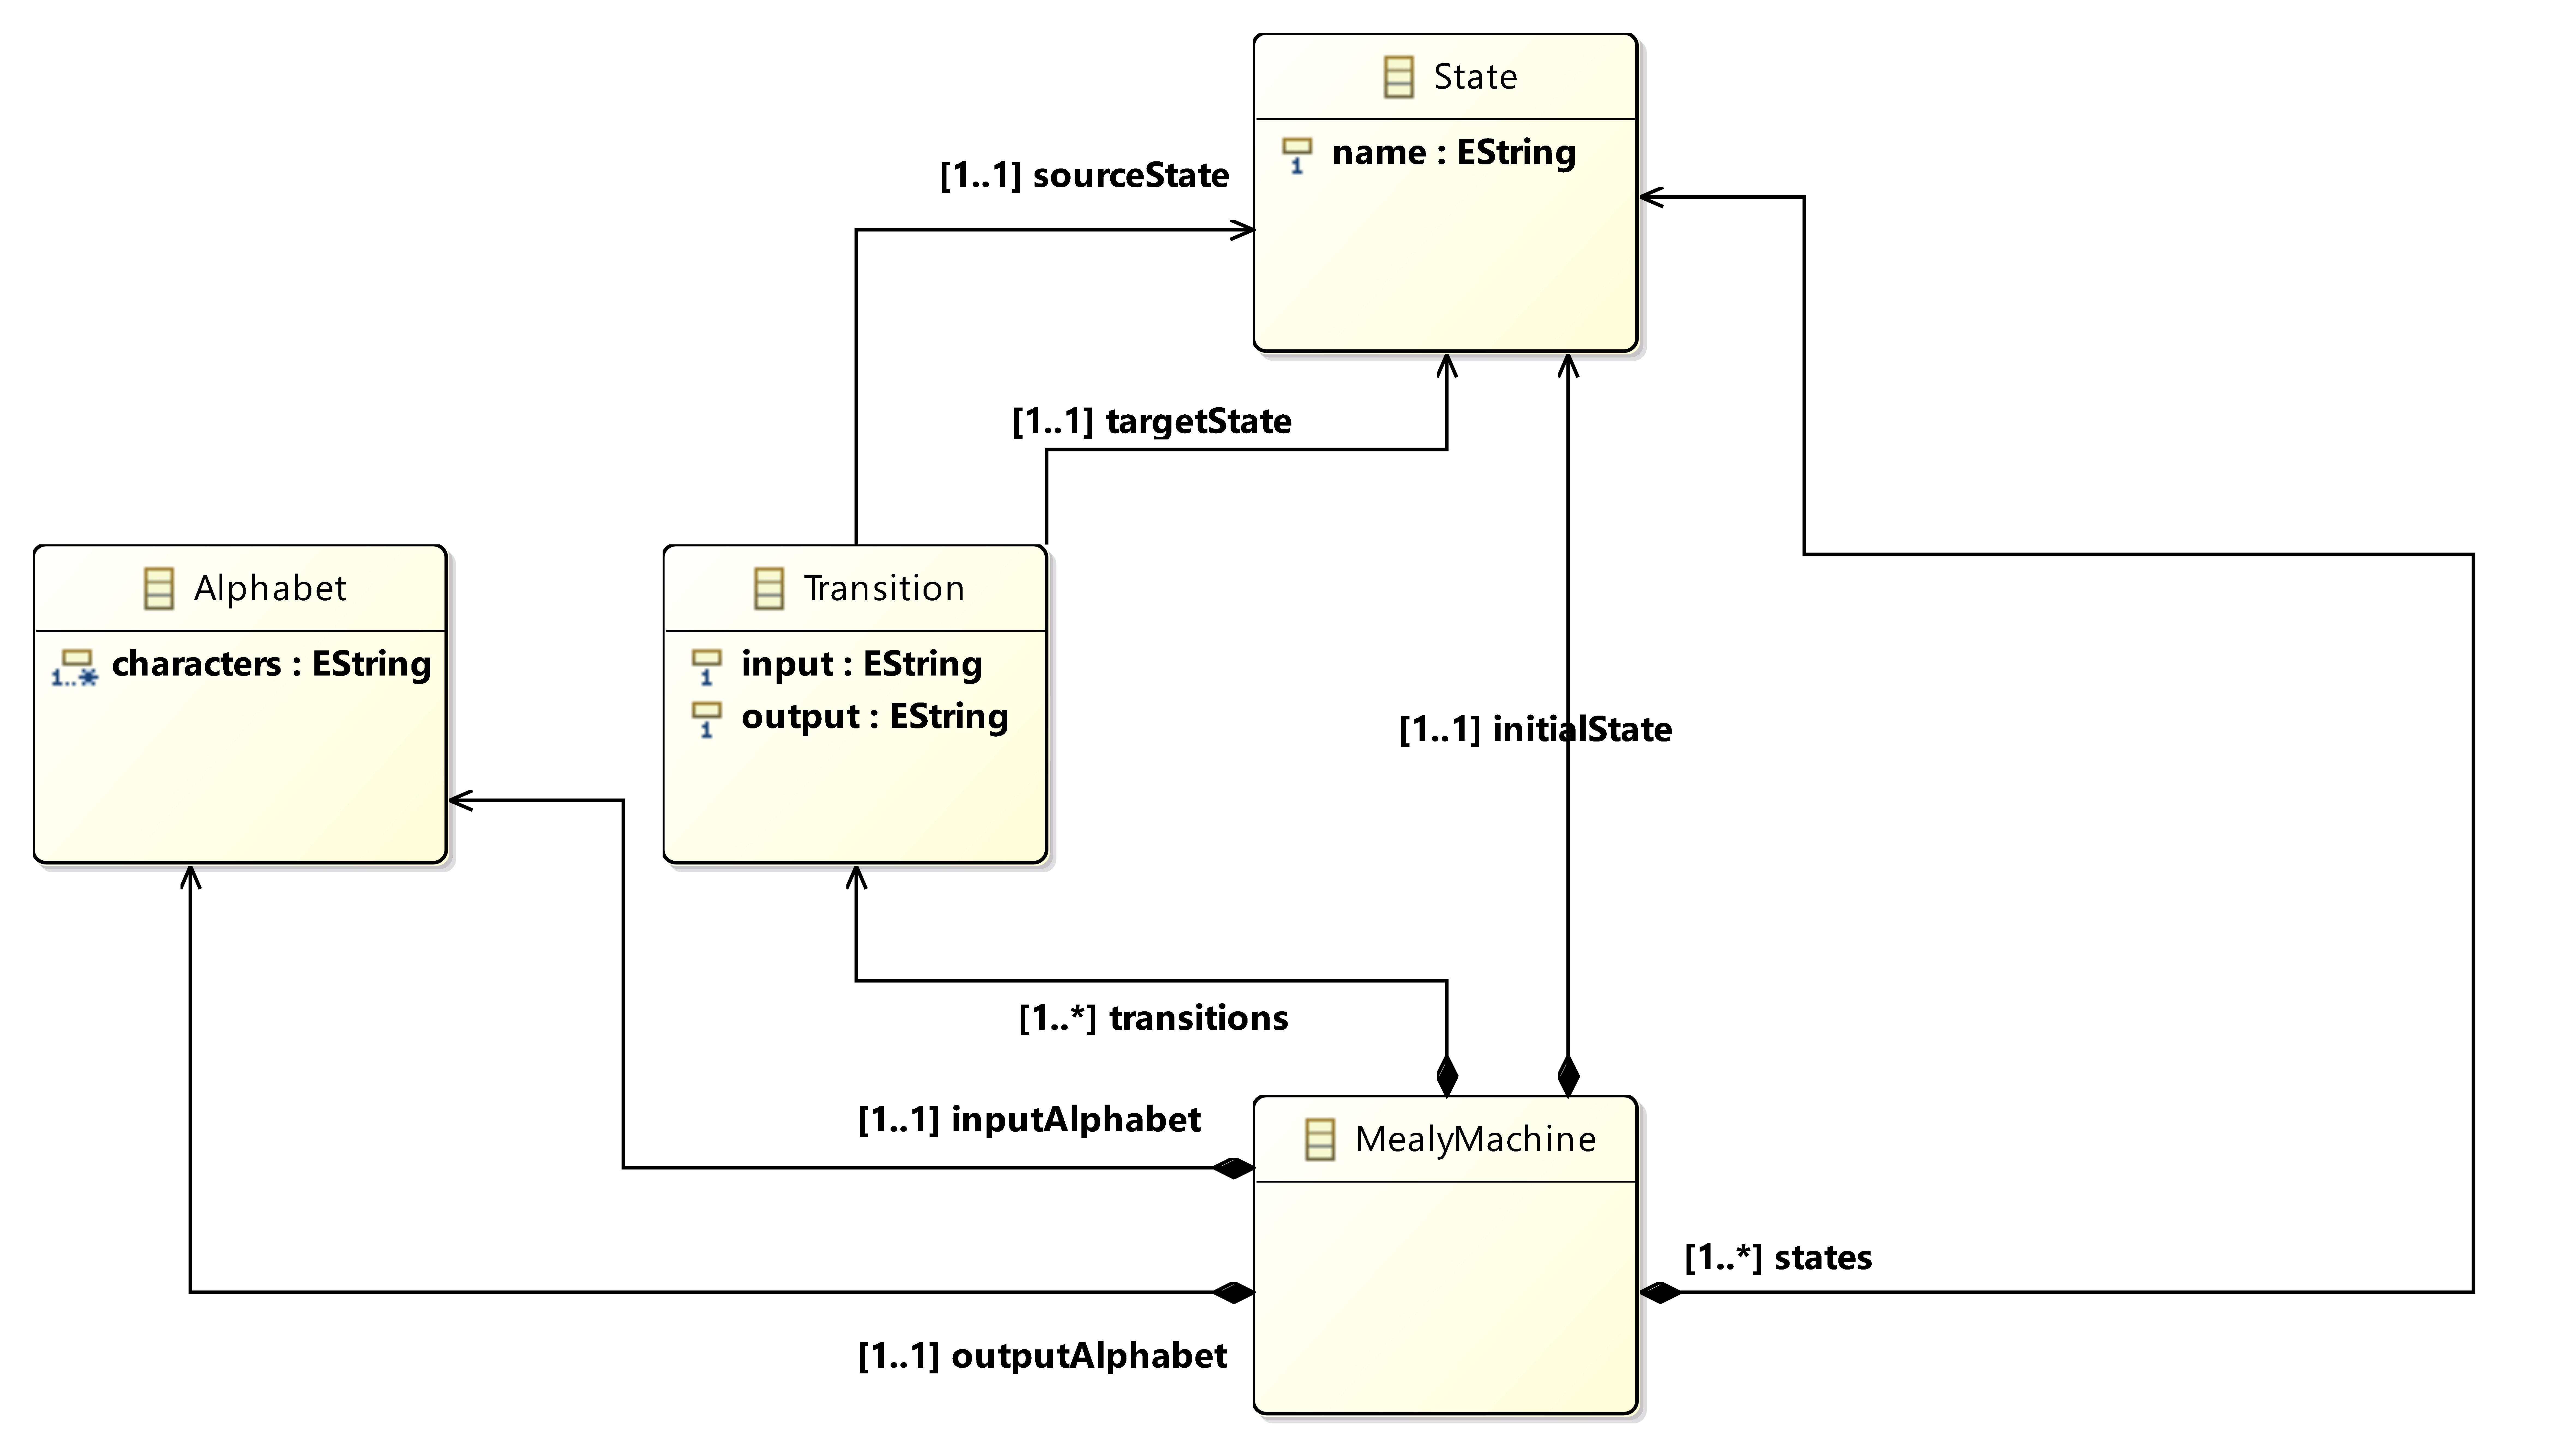
\includegraphics[width=1.0\linewidth]{figures/mealymodel}
	\caption{Ecore metamodel of Mealy machines.}
	\label{fig:mealyecore}
\end{figure}

In text, the Ecore model uses Strings as distinguishers (on code generation, EString is converted to java.lang.String). States of the automaton, i.e. State objects are differentiated based on the name field. Note, that this is a transition-driven model of Mealy machines, the Transition class has a reference to the source and target states of the transition, as opposed to some models, where states store their own transition information (successors, predecessors) like nodes in a graph. This decision was based on the DHC algorithm, which stores traversal information itself, rather than asking for it, which is why ease of access is preferred as opposed to efficiency.

Extending upon the metamodel in Figure \ref{fig:mealyecore}, I generated the Xtext grammar seen in Listing \ref{li:xtext} utilizing Xtexts EMF integration. In words, this  grammar describes a textual grammar in which instances of the metamodel seen in Fig. \ref{fig:mealyecore} can be stored. 



\begin{lstlisting}[caption=Xtext grammar describing Mealy machines.,label=li:xtext,float,floatplacement=H]
MealyMachine returns MealyMachine:
'MealyMachine'
'{'
'initialState' initialState=State
'states' '{' states+=State ( "," states+=State)* '}' 
'inputAlphabet' inputAlphabet=Alphabet
'outputAlphabet' outputAlphabet=Alphabet
'transitions' '{' transitions+=Transition ( "," transitions+=Transition)* '}' 
'}';

State returns State:
{State}
'State'
name=EString;

Alphabet returns Alphabet:
'Alphabet'
'{'
'characters' '{' characters+=EString ( "," characters+=EString)* '}' 
'}';

Transition returns Transition:
'Transition'
'{'
'input' input=EString
'output' output=EString
'sourceState' sourceState=[State|EString]
'targetState' targetState=[State|EString]
'}';

EString returns ecore::EString:
STRING | ID;
\end{lstlisting}

An example of a MealyMachine instance in the form if the grammar in Listing \ref{li:xtext} can be seen in Listing \ref{li:4ixtext}.

\begin{lstlisting}[caption=The Mealy machine seen in Fig.\ref{fig:dfaexamplemealyver}.a in the form of the Xtext grammar described in Listing \ref{li:xtext}.,label=li:4ixtext]
MealyMachine{
initialState 
State q0 states { State q0, State q1, State q2, State q3}
inputAlphabet Alphabet { characters { a , b } }
outputAlphabet Alphabet { characters { top , bot } }
transitions{ 
Transition { input a output top sourceState q0 targetState q1 } , 
Transition { input b output top sourceState q0 targetState q0 } , 
Transition { input a output top sourceState q1 targetState q2 } , 
Transition { input b output top sourceState q1 targetState q1 } , 
Transition { input a output bot sourceState q2 targetState q3 } , 
Transition { input b output top sourceState q2 targetState q2 } , 
Transition { input a output top sourceState q3 targetState q0 } , 
Transition { input b output bot sourceState q3 targetState q3 } } }
\end{lstlisting}


\subsection{Direct Hypothesis Construction}

While implementing the DHC algorithm, I used the above described MealyMachine formalism using the Xtext input source (later seen as \emph{MealyMachineLearnable}), but I also described a way to programmatically describe an input to ease the process of creating small inputs (later seen as \emph{StringSequenceLearnable}). Both are expanded upon in the following.





\label{item:stringsequencelearnable}

The detailed (but not exhaustive) class diagram of the frameworks DHC implementation can be seen in Fig. \ref{fig:impldetailedoverview}. The figure is self-explanatory in some regards, while the generic specifics and implementation details are explained in the following.

\begin{itemize}
	\item \textbf{StringSequenceLearnable:} The \emph{StringSequenceLearnable} class is a realization of the Learnable interface, defining simply any type of learnable, which use Strings (java.lang.String) as both input and output types. It contains a simple implementation for describing behavior, accepting a String in the format of $"|input1|output1|input2|output2|...|inputn|outputn|"$, and storing it in a HashMap. One example of this formalism can be seen in Fig. \ref{fig:alternatingbit}.
	
	\item \textbf{MealyLearnable:} The \emph{MealyLearnable} class is a \emph{Learnable} which uses the EMF-modeled \emph{MealyMachine} class seen in Fig. \ref{fig:mealyecore}. Since this implementation of Mealy machines uses Strings as both input and output characters, it extends upon the generic bounds provided by the \emph{StringSequenceLearnable} class.
	
	\item \textbf{DHCHypothesis:} The \emph{DHCHypothesis} abstract class contains the abstractions the DHC algorithm needs to be separated from the implementation of the output formalism. Output here is also implementation-dependent, for DFAs it would be the state after running an input, for Mealy machines it would be output after running an input. Contrary to the \emph{Adapter} layer of input formalisms, every algorithm must define its own abstract hypothesis type, an example being this (the \emph{DHCHypothesis}) class.
	
	\item \textbf{DHCMealyMachineHypothesis:} The \emph{DHCMealyMachineHypothesis} class straightforwardly extends \emph{DHCHypothesis} using the EMF-modeled \emph{MealyMachine} class seen in Fig. \ref{fig:mealyecore}. Essentailly, \emph{DHCMealyMachineHypothesis} is the Mealy machine extension of the DHCHypothesis abstract class, implementing every abstract method of both its superclasses.
	
	\item \textbf{StringSequenceAdapter:} The \emph{StringSequenceAdapter} abstract class adapts \emph{StringSequenceLearnable}s (bounds these using generics), while not defining any generic bounds to the \emph{Hypothesis} it adapts to. This makes it possible to implement equivalance queries only once for every input formalism, using the abstract \emph{convert...()} methods to be implemented by subclasses. The current implementation uses a brute-force method of comparing the outputs of the \emph{Learnable} and the \emph{Hypothesis} for every possible input under the input alphabet. This implementation can be seen in \ref{li:eqbruteforce}.
	
	\item \textbf{StringSequenceToMealyAdapter:} The \emph{StringSequenceToMealyAdapter} class bounds the \emph{Hypothesis} parameters of the \emph{LearnableAdapter} to \emph{DHCMealyMachineHypothesis}, as the dependency relation indicates in Fig. \ref{fig:abstractdetailedoverview}. It only implements the \emph{convert...()} functions.

	\item \textbf{MealyMachineTeacher:} The \emph{MealyMachineTeacher} abstract class bounds the generic parameters of the \emph{Hypothesis} (H) to \emph{DHCMealyMachineHypothesis}, while leaving the \emph{Learnable} (LA) parameter unbound, analogously to \emph{StringSequenceAdapter}. This is done, so algorithm implementations are completely separated from input types. 
	\item \textbf{MealyMachineTeacherStringSequenceImpl:} The \emph{MealyMachineTeacherStringSequenceImpl} class defines the LA generic parameter to be a \emph{StringSequenceAdapter}, and delegates both its methods to it.
	 
	\item \textbf{DirectHypothesisConstruction:} The \emph{DirectHypothesisConstruction} class implements the DHC algorithm using the \emph{DHCHypothesis} abstract class to build its hypothesis. The \emph{constructHypothesis()} method is an implementation of Algorithm \ref{algo:dhc}, constructing a \emph{DHCHypothesis} in a black-box way using the splitters field. The splitters field is initialized and constructed the way described in Algorithm \ref{algo:dhc}, on the first run initialized by the input alphabet, then extended on hypothesis refinement. The \emph{refineHypothesis()} method does exactly this: it takes a counterexample, and adds the suffixes of it to the \emph{splitters}, so the next run of \emph{constructHypothesis()} will split states as needed. The \emph{execute()} method ties everything together by executing \emph{constructHypothesis()}, equivalence queries and the \emph{refineHypothesis()} method. The implementation of the \emph{execute()} method can be seen in Listing \ref{li:executedhc}.\\

	
	\begin{figure}[H]
		\centering

		\centerline{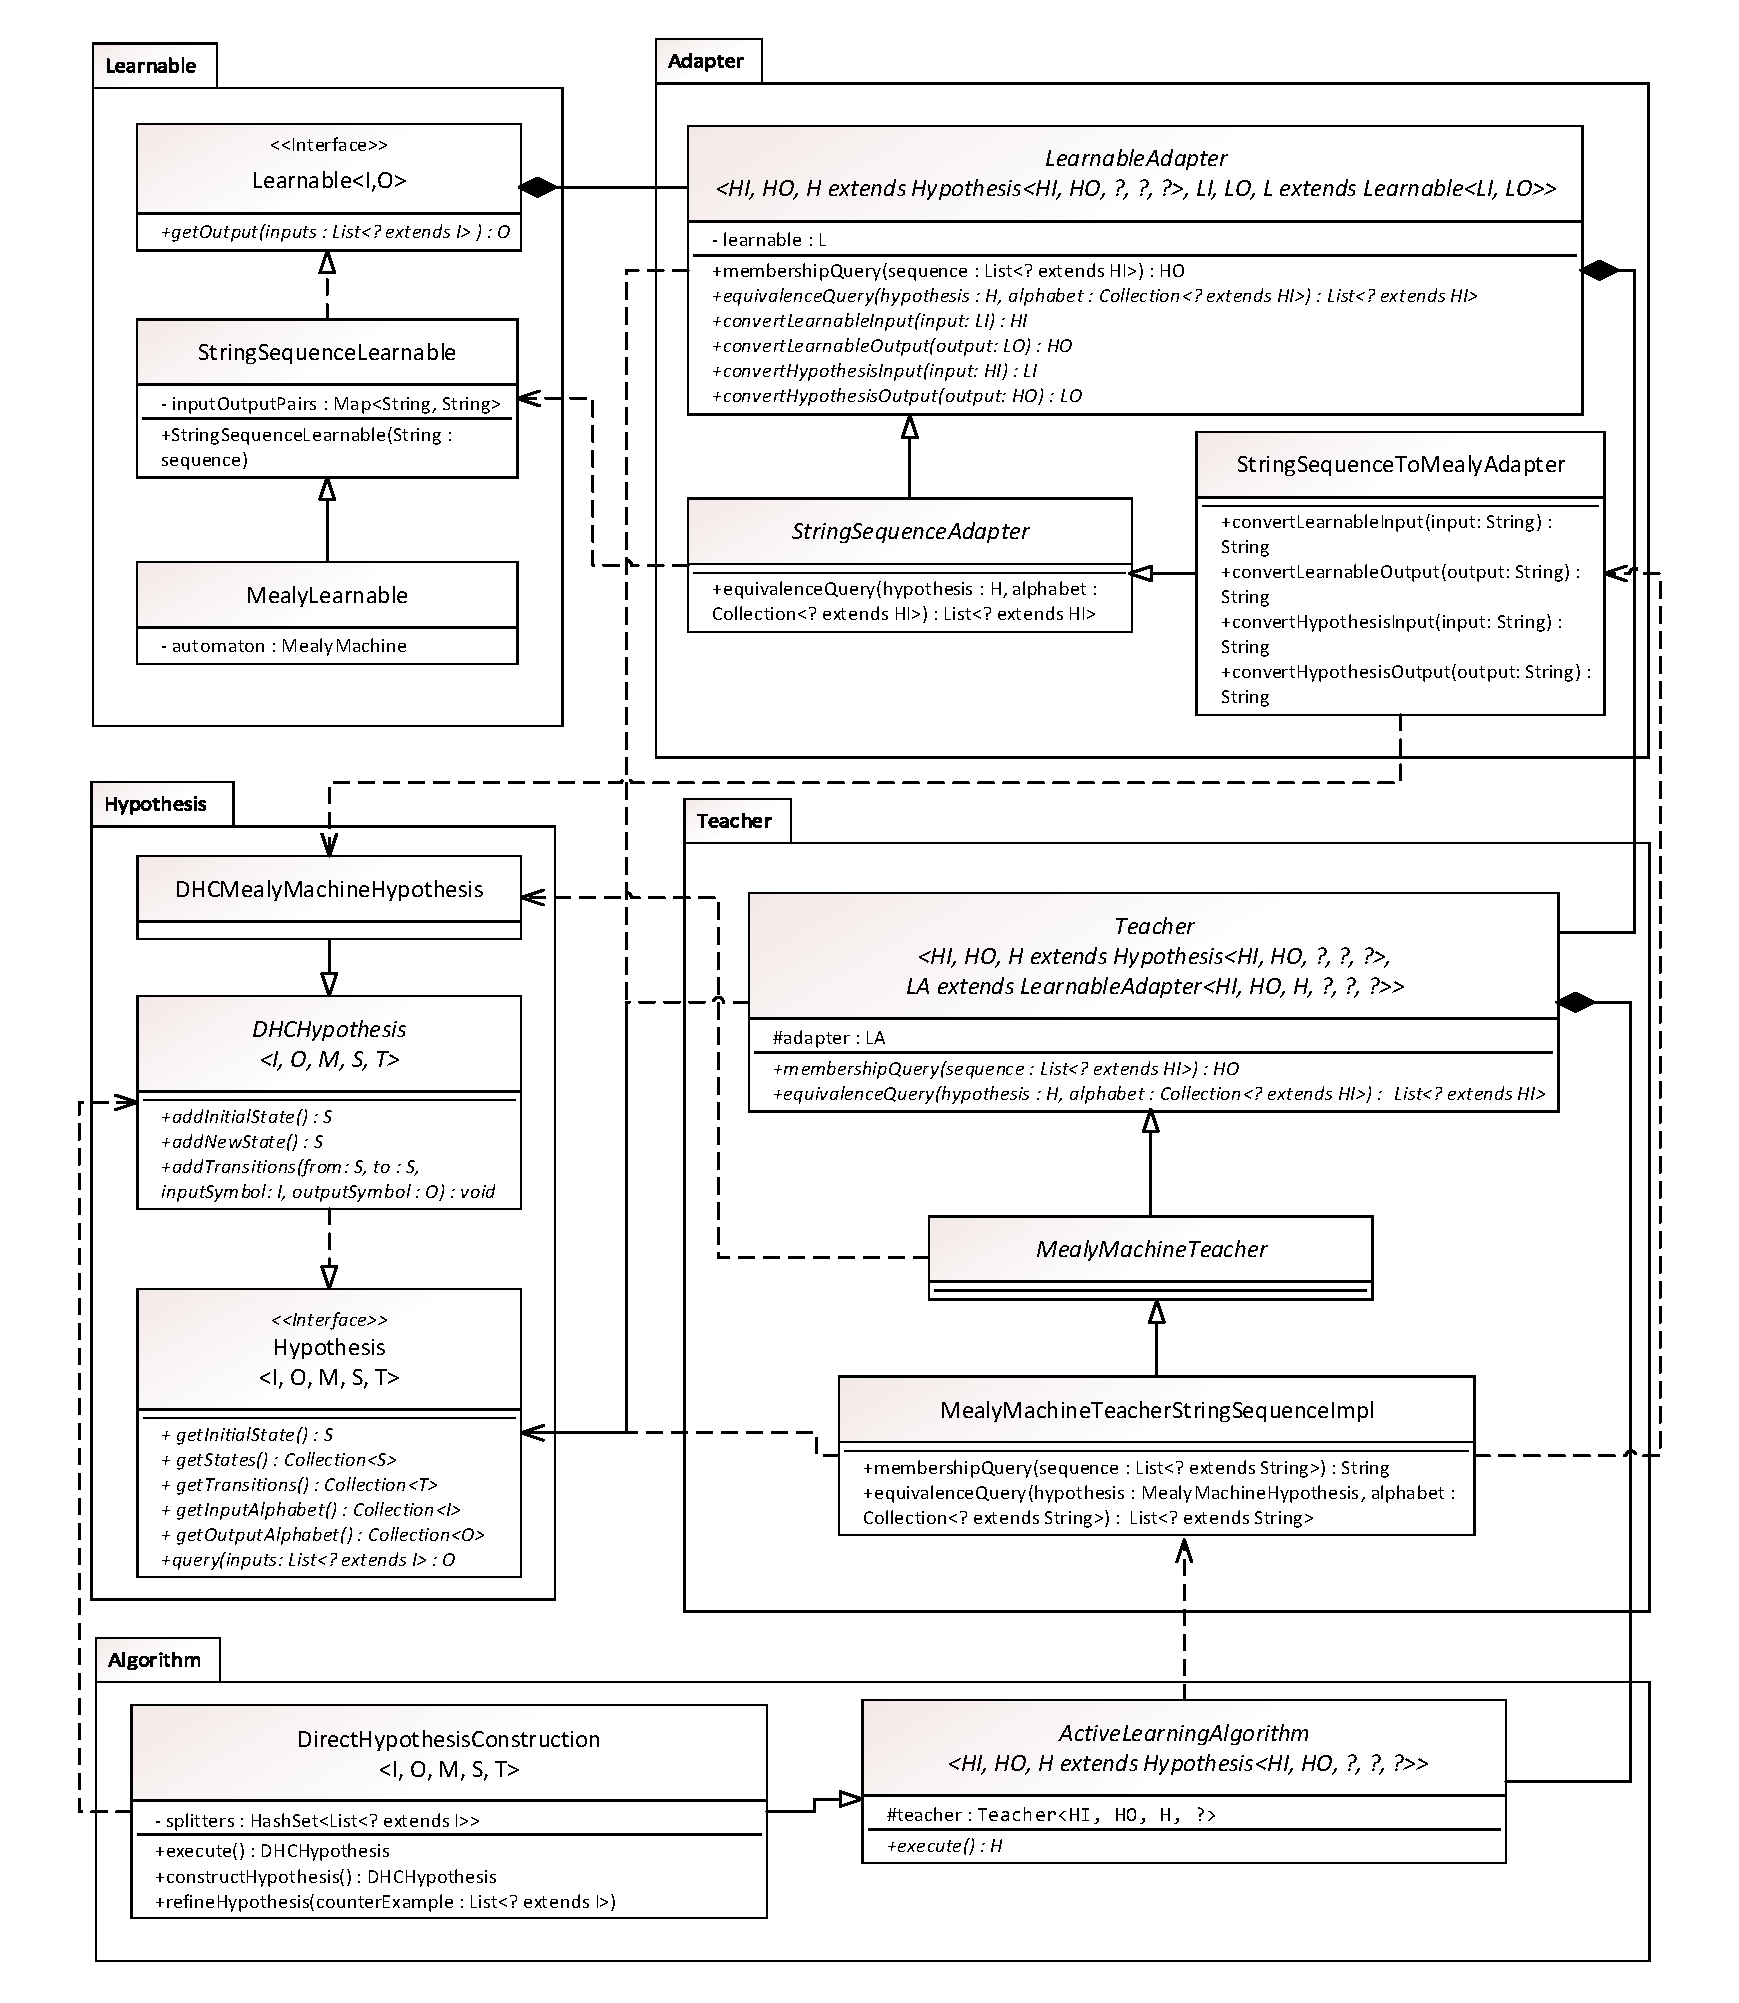
\includegraphics[width=.90\paperwidth,height=.90\paperheight,keepaspectratio]{figures/implementationdetailedoverview}}
		\caption{Non-exhaustive detailed structural overview of the frameworks DHC implementation.}
		\label{fig:impldetailedoverview}
	\end{figure}
	
	
	
	\begin{lstlisting}[caption=The \emph{execute()} function of the DHC algorithm implementation described in Section \ref{item:stringsequencelearnable}s \emph{DirectHypothesisConstruction} item.,label=li:executedhc,float,floatplacement=H]
public DHCHypothesis execute() {
	List<? extends I> counterExample = null;
	DHCHypothesis<I, O, M, S, T> h = null;
	do {
		if(counterExample != null) {
			refineHypothesis(counterExample);
		}
		h = constructHypothesis();
		
		counterExample = teacher.equivalenceQuery(h, alphabet);
	}while(counterExample != null);
	
	return h;
}
	\end{lstlisting}
	Note, that the implementatation utilizes the DHCHypothesis abstract class, providing a separation of the DHC algorithm and the output formalism it constructs while learning.

\end{itemize}



\subsection{TTT}

The TTT algorithm is complex, in both theory and implementation. Due to it using multiple specific types of data structures and sub-algorithms, which are not themselves part of TTT, during my imlementation I depended on the original (defining) implementation of it in LearnLib\cite{10.1007/978-3-319-21690-4_32}.
\\
LearnLib describes an abstract layer of TTT to extend in implementations. I used these abstractions to implement the algorithm into my framework in an (from the perspective of execution) almost seamless manner. The current implementation only allows MealyMachines as inputs, but this can be extended upon analogously as with the DHC implementation seen previously.

The implementation itself is built similarly as the DHC implementation, but the algorithm wraps the abstractions of the framework and converts between types of these abstractions and the ones used in LearnLib. More specifically, LearnLib defines abstract types for parts of the TTT algorithms, such as \emph{AbstractTTTHypothesis},\emph{AbstractBaseDTNode} (abstract discriminator tree node), \emph{AbstractTTTLearner}. While LearnLib has implementations of these, I only depended on abstractions, using the current implementation as reference.
\\\\
For key steps of TTT, the responsibilities of the current implementation are as follows. The Hypothesis construction and refinement is done by my framework, which provides the methods of hypothesis construction, while also hadling the calculation of output inconsistencies and the refinement of them. LearnLib manages the internal data structures including the dicriminator tree, which stores my implementation of the $AbstractBaseDTNode$ class. The state splitting (part of Hypothesis stabilization) and discriminator finalization is handled by LearnLib. Considering the communication with the system under learning, equivalence queries are done in the exact way presented in the DHC algorithm, done by wrapping the \emph{Teacher} class of my implementation into the \emph{EquivalenceOracle} interface of LearnLib. The same solution could not be used with membership queries, since the TTT algorithm internally tries avoiding these queries (done partly by finding output inconsistencies), and has specific behavior in its LearnLib implementation differing from traditional membership queries. The conversion between the formalisms used by the two frameworks allowed me to natively use their \emph{MembershipOracle} interface with the converted \emph{Learnable}.



\subsection{Case studies}

\renewcommand{\tabularxcolumn}[1]{m{#1}}
\newcolumntype{Y}{>{\centering\arraybackslash}X}
\begin{table}[H]
	
	\begin{tabularx}{\columnwidth}{YYYYY}
		\hline
		\textbf{Algorithm} & \textbf{Input formalism} & \textbf{Output formalism} & \textbf{Input source} & \textbf{Output source}\\ \hline
		DHC & Mealy machine & Mealy machine & Xtext & Xtext 
		\\	\hline
		DHC & String sequences & Mealy machine & String & Xtext
		\\ \hline
		TTT & Mealy machine & Mealy machine & Xtext & Xtext 
		\\	\hline
	\end{tabularx}
	\caption{Overview of the algorithm implementations in the framework.}
	\label{tab:activelearningproto}
\end{table}

A summary of the DHC and TTT implementations can be seen in Table \ref{tab:activelearningproto}.

After running the example seen in Listing \ref{li:4ixtext}, the output of the DHC algorithm can be seen in Listing \ref{li:xtextdhc}, while the output of the TTT algorithm can be seen in Listing \ref{li:xtextttt}. As a case study, both these algorithms were ran on the Mealy machine seen in Fig. \ref{fig:coffeemealy} contained in the input seen in Listing \ref{li:coffeemealy}, resulting in the outputs Listing \ref{li:coffeetttret} and Listing \ref{li:coffeedhcret} repsectively.
\chapter{Evaluation}

\section{Theoretical evaluation}

The framework presented in this thesis has both advantages and disadvantages in design and implementation. The modular setup shown in Fig. \ref{fig:abstractoverview}, while providing easy extensibility, does require knowledge of the algorithms implemented therein. In contrary to LearnLib, where (from my experience) data structures are easily extended and onboarded to the learning, algorithm implementations are difficult to provide new solutions to, my framework allows extensibility on every front of it, with a steeper learning curve even with new input/output onboarding. This makes the framework optimal from an engineering perspective, since it allows the integration of other tools. For example, through the implemented EMF formalism, both the Gamma Statechart Composition framework\cite{DBLP:conf/icse/MolnarGVMV18} and the Theta framework\cite{theta-fmcad2017} can be integrated in the future.

The framework, when implementing similar formalisms does require some redundancy, especially with the \emph{Learnable-LernableAdapter-Teacher} trio of implementation needed with new formalisms. The advantage of this sometimes redundant approach is the overall elimination of typecasting and uncertain genericity, allowing for exact application of methods and classes after bounding the generic parameters required, improving runtime, the compliance with object-oriented paradigms, and understandibility of an implementation without context of its abstrations. The \emph{Learnable} and \emph{Hypothesis} endpoints of input and output formalisms being interfaces provide flexibility by leveraging the multiple-inheritance (implementation) property of interfaces. This is used for example in the TTT implementation in order to extend upon classes of LearnLib, while still implementing my frameworks abstractions.

\subsection{Evaluation of DHC}

The Direct Hypothesis Construction algorithm, as theorized and proved in \cite{Steffen2011} and \cite{10.1007/978-3-642-34781-8_19}, terminates after at most $n^3mk+n^2k^2$ membership, and $n$ equivalence queries, where $n=|S|$, $k=|\Sigma|$ and $m$ is the longest counterexample. The runtime complexity of these queries are difficult to evaluate, since they highly depend on implementation and context. Reaching the system under learning in the current implementation of input formalisms (String sequece or Mealy machine) takes no overhead, since the system behavior is stored in-memory. This might not be the case in other implementations, where the SUL might be reached through network communication or other methods with non-negligible overhead. In terms of membership queries, the current implementations differ. 

String sequences (\emph{StringSequenceLearnable}s) are stored in an input-output \emph{HashMap}, which allows $O(1)$ access assuming the values are evenly distributed in the buckets used by the hashing, worst-case scenario being $O(k)$. While access is fast, this method suffers in terms of space complexity, storing a numer of elements identical to $\mathcal{P}(\Sigma)\setminus\emptyset$, or in text, the powerset of $\Sigma$ without the empty set, resulting in a space complexity of $O(2^k)$.

The MealyMachine implementation (the \emph{MealyLearnable} class) provides a more reasonable $O(k)$ space complexity, but it struggles with runtime issues. This transition-driven implementation of Mealy machines, as discussed in Chapter \ref{contrib}, provides ease of access to the automaton, resulting in a straightforward implementation of membership queries. However, not storing the automata in a graph-like format reduces efficiency. This results in a worst-case scenario of $O(kt)$, where $t$ is the number of transitions of the automaton.

From the perspective of equivalence queries, the two implemented input formalisms both provide the same efficiency. Since the implementation of this query is in the \emph{StringSequenceAdapter} class, both \emph{MealyLearnable} and \emph{StringSequenceLearnable} are queried using this implementation, which can be seen in Listing \ref{li:eqbruteforce}. This implementation is a brute-force way of proving equivalence of the hypothesis and the system under learning, operating by taking every permutation of every element in $\mathcal{P}(\Sigma)\setminus\emptyset$ and comparing outputs using membership queries for each of them. In order to mitigate some of this inefficiency, the implementation uses google guavas \emph{Sets.powerSet()} method, providing $O(k)$ space complexity as opposed to a brute-force $O(2^k)$ implementation. For each member of $\mathcal{P}(\Sigma)\setminus\emptyset$, the permutations are calculated using the \emph{Collections2.permutations()} method of guava, implementing the Johnson–Trotter algorithm. This results in a $O(2^kk!)$ number of membership queries considering the "worst case" of finding no counterexamples.

In summary, the best-case scenario of the current DHC implementation has an $O(n^3mk^2+n^2k^3+2^kk!k)$ runtime complexity, and the worst case is $O(n^3mk^2t+n^2k^3t+2^kk!kt)$ depending on the variables presented above.

\subsection{Evaluation of TTT}

The TTT algorithm, as presented in \cite{10.1007/978-3-319-11164-3_26}, requires $O(n)$ equivalence queries and $O(kn^2+n\log m)$ membership queries, each of which takes $O(n+m)$ time, where $n=|S|$, $k=|\Sigma|$ and $m$ is the longest counterexample. This is a very pessimistic estimate caused by the edge-case of a discriminator tree having a height of $n$. The time complexity of the equivalence query implementation seen in \ref{li:eqbruteforce} still holds as $O(2^kk!)$, but is lengthened by the complexity of conversion between formalisms, being $O(nt)$ in the worst case, where $t$ is the number of transitions of the current hypothesized automaton. Altogether, the worst case scenario has a $O((kn^2+n\log m)(n+m) + 2^kk!nt)$ time complexity. TTT also provides an efficient $\Theta(kn)$ space complexity\cite{10.1007/978-3-319-11164-3_26}.


\section{Experimental evaluation}

The experimental evaluation of the implemented algorithms were performed using variations of the automaton seen in Fig. \ref{fig:dfaexamplemealyver}.a. This decision is based on the simplicity of extending the automaton accepting inputs containing $4i+3a$ to inputs containing $ni+(n-1)a$, where $n\in \mathbb{N}$ is the size of the loop in the automaton and $i \in \mathbb{N}$. An example of this can be seen in Fig. \ref{fig:5ia}, where $n=5$. This solution is easily scalable and straightforward to implement even for large $n$-s.

\begin{figure}
	\centering
	\begin{tikzpicture}[shorten >=1pt,node distance=3.5cm,on grid,auto] 
	\node[state,initial] (q_0)   {$q_0$}; 
	\node[state] (q_1) [right=of q_0] {$q_1$}; 
	\node[state] (q_2) [below=of q_0] {$q_2$}; 
	\node[state](q_3) [right=of q_2] {$q_3$};
	\node[state](q_4) [above right= 2.4cm of q_3] {$q_4$};
	\path[->] 
	(q_0) edge[]  node {a/$\top$} (q_1)
	edge [loop below] node {b/$\top$} ()
	(q_1) edge[]  node[pos=0.62]  {a/$\top$} (q_2)
	edge [loop below] node {b/$\top$} ()
	(q_2) edge[]  node [swap] {a/$\top$} (q_3) 
	edge [loop above] node {b/$\top$} ()
	(q_3) edge  node[pos=0.62] [swap] {a/$\bot$} (q_4)
	edge [loop above] node {b/$\top$} () 
	(q_4) edge[bend right=70]  node[pos=0.62] [swap] {a/$\top$} (q_0)
	edge [loop right] node {b/$\bot$} ();
	
	\end{tikzpicture}
	\caption{Example of an automaton accepting inputs containing $5i+4a$.}
	\label{fig:5ia}
\end{figure}

As seen in the theoretical evaluation, the size of the state space is not the only possible bottleneck, both algorithms (and the equivalence query implementation especially) slow with the size of the input alphabet. A simple solution of testing growing input alphabets using the Mealy machine seen in Fig. \ref{fig:dfaexamplemealyver}.a, is to add characters (transitions) without adding behavior. This does not remove the minimal property of an automaton, contrary to adding states without changing behavior, thus increasing runtime. An example of the described input alphabet extension can be seen in Figure \ref{fig:abcextended}.

\begin{figure}
	\centering
	\begin{tikzpicture}[shorten >=1pt,node distance=3.5cm,on grid,auto] 
	\node[state,initial] (q_0)   {$q_0$}; 
	\node[state] (q_1) [right=of q_0] {$q_1$}; 
	\node[state] (q_2) [below=of q_0] {$q_2$}; 
	\node[state](q_3) [right=of q_2] {$q_3$};
	\path[->] 
	(q_0) edge[]  node {a/$\top$} (q_1)
	edge [loop below] node {b/$\top$} ()
	edge [loop above] node {c/$\bot$} () 
	(q_1) edge[]  node[pos=0.62]  {a/$\top$} (q_2)
	edge [loop below] node {b/$\top$} ()
	edge [loop above] node {c/$\bot$} () 
	(q_2) edge[]  node [swap] {a/$\top$} (q_3) 
	edge [loop above] node {b/$\top$} ()
	edge [loop below] node {c/$\bot$} () 
	(q_3) edge  node[pos=0.62] [swap] {a/$\bot$} (q_0)
	edge [loop above] node {b/$\bot$} () 
	edge [loop below] node {c/$\bot$} () ;
	\end{tikzpicture}
	\caption{Example of the automaton seen in Fig. \ref{fig:dfaexamplemealyver}.a with an extended input alphabet $\Sigma=\{a, b, c\}$.}
	\label{fig:abcextended}
\end{figure}

Table \ref{tab:evalspecs} details the specifications on which the measurements were ran.

\renewcommand{\tabularxcolumn}[1]{m{#1}}
\newcolumntype{Y}{>{\centering\arraybackslash}X}
\begin{table}[H]
	
	\begin{tabularx}{\columnwidth}{YYYYY}
		\hline
		\textbf{Operating system} & \textbf{Processor}  & \textbf{Java version} & \textbf{Eclipse version} & \textbf{Heap size} \\ \hline
		Windows 10 Pro & Intel Core i7-8700 & OpenJDK 1.8 & Eclipse Modeling Tools 4.12.0 & Xms1024m, Xmx2048m
		\\ \hline
	\end{tabularx}
	\caption{Overview of the algorithm implementations in the framework.}
	\label{tab:evalspecs}
\end{table}

After running the experiments, an obvious bottleneck could be found. The current brute-force equivalence query implementation is inefficient, as the theoretical evaluation suggested. Figure \ref{fig:stateruntime} shows the inefficiency observed when extending the states and the behavior of the learned automaton. Similarly, the TTT implementation was slowed to the point of having the same runtime as the DHC algorithm, as illustrated by Fig. \ref{fig:stateruntimettt}. The same can be said about the extenstion of the input alphabet, Fig. \ref{fig:inputruntime} and Fig. \ref{fig:inputruntimettt} show the DHC and the TTT algorithms respectively being bottlenecked to the point of indifferentiability. This is caused by both the inefficient equivalence query and the small size of the automata being learned. 

It is important to note, that these inefficiencies were not caused by the learning algorithms, but by the equivalence algorithm. In order to remove the bottleneck and compare the actual learning algorithm runtimes, an optimized, near linear-time equivalence oracle from \emph{LearnLib} was onboarded to the framework for both the DHC and TTT algorithms to use.

Figure \ref{fig:stateruntimeopt} and Figure \ref{fig:stateruntimeoptttt} show the runtime of the DHC and the TTT algorithms for growing state spaces. The difference in efficiency is obvious, while DHC learned a 344 state automaton for two and a half minutes, TTT learned the automaton accepting $1904i-1903a$ (which contains 1904 states) in the same time. Similar results can be seen in Fig. \ref{fig:inputruntimeopt} and Fig. \ref{fig:inputruntimeoptttt}, which illustrate, that DHC depends on the size of the input alphabet vastly more, than TTT does.

\begin{figure}
	\centering
	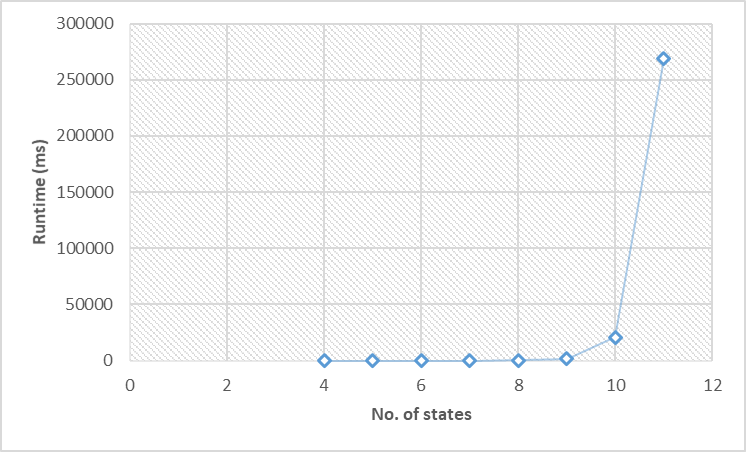
\includegraphics[width=0.7\linewidth]{figures/stateruntime}
	\caption{The bottleneck the brute-force equivalence query implementation causes when increasing the state space while running DHC.}
	\label{fig:stateruntime}
\end{figure}

\begin{figure}
	\centering
	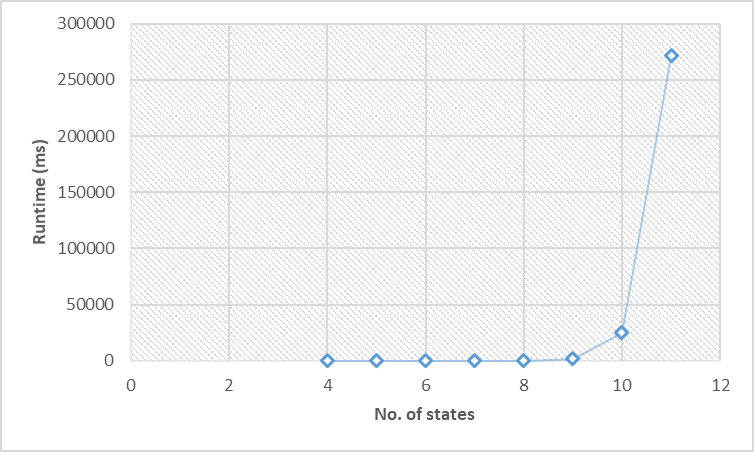
\includegraphics[width=0.7\linewidth]{figures/stateruntimettt}
	\caption{The bottleneck the brute-force equivalence query implementation causes when increasing the state space while running TTT.}
	\label{fig:stateruntimettt}
\end{figure}

\begin{figure}
	\centering
	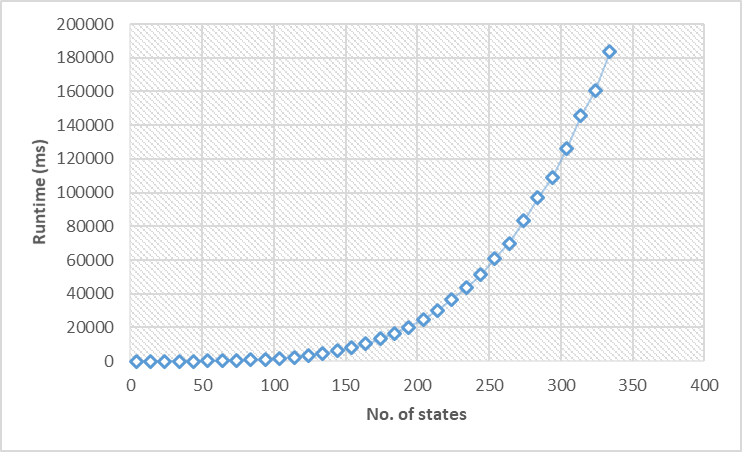
\includegraphics[width=0.7\linewidth]{figures/stateruntimeopt}
	\caption{Runtime of the DHC algorithm with increasing state space using the optimized equivalence query from \emph{LearnLib}.}
	\label{fig:stateruntimeopt}
\end{figure}


\begin{figure}
	\centering
	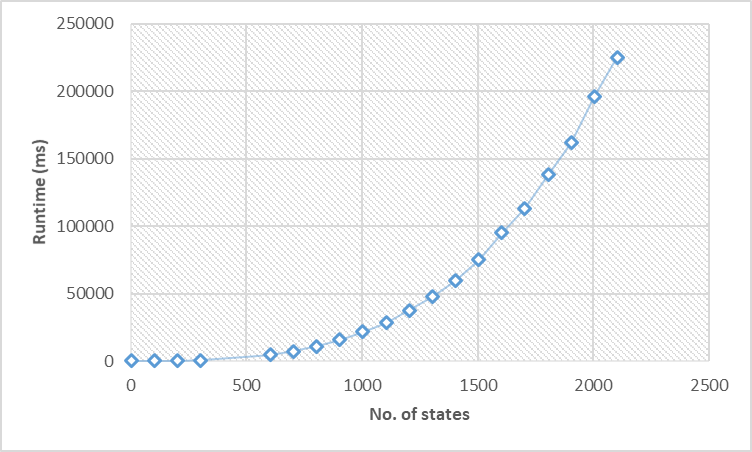
\includegraphics[width=0.7\linewidth]{figures/stateruntimeoptttt}
	\caption{Runtime of the TTT algorithm with increasing state space using the optimized equivalence query from \emph{LearnLib}.}
	\label{fig:stateruntimeoptttt}
\end{figure}



\begin{figure}
	\centering
	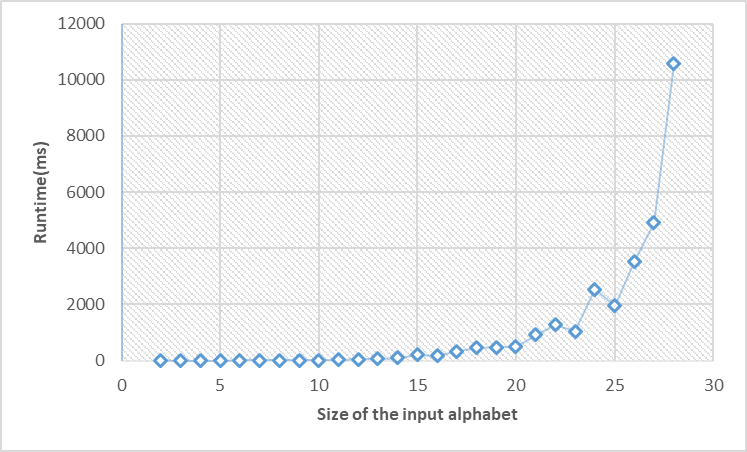
\includegraphics[width=0.7\linewidth]{figures/inputruntime}
	\caption{The bottleneck the brute-force equivalence query implementation causes when increasing the input alphabet while running DHC.}
	\label{fig:inputruntime}
\end{figure}

\begin{figure}
	\centering
	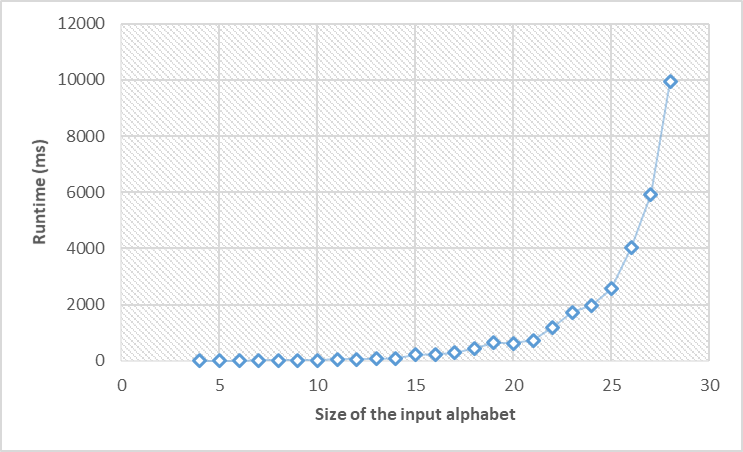
\includegraphics[width=0.7\linewidth]{figures/inputruntimettt}
	\caption{The bottleneck the brute-force equivalence query implementation causes when increasing the input alphabet while running TTT.}
	\label{fig:inputruntimettt}
\end{figure}

\begin{figure}
	\centering
	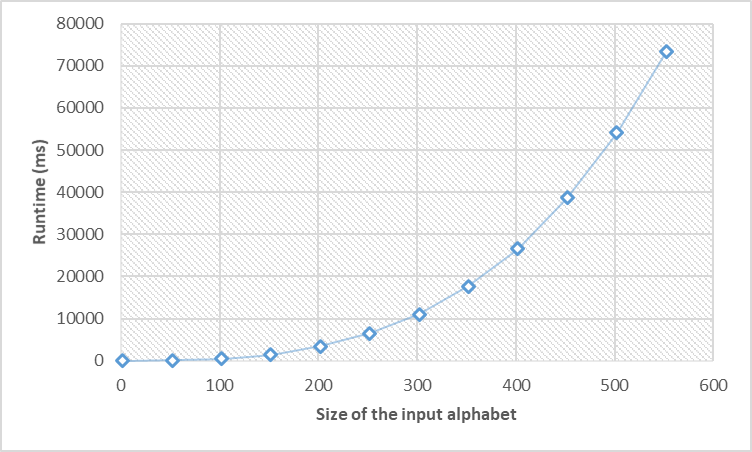
\includegraphics[width=0.7\linewidth]{figures/inputruntimeopt}
	\caption{Runtime of the DHC algorithm with increasing input alphabet using the optimized equivalence query from \emph{LearnLib}.}
	\label{fig:inputruntimeopt}
\end{figure}


\begin{figure}[H]
	\centering
	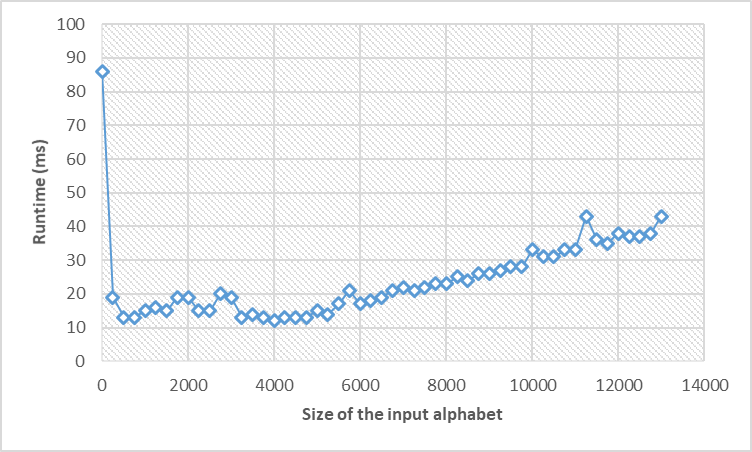
\includegraphics[width=0.7\linewidth]{figures/inputruntimeoptttt}
	\caption{Runtime of the TTT algorithm with increasing input alphabet using the optimized equivalence query from \emph{LearnLib}.}
	\label{fig:inputruntimeoptttt}
\end{figure}

In summary, for smaller system components, the DHC algorithm is straightforward to use, formalisms are also simple to onboard to it. However, for most use cases in system design, the efficiency of the TTT algorithm overweigh the implementation complexity of it, making the TTT the better solution for most practical problems.


\chapter{Conclusions}
This chapter concludes the contributions of this thesis, and presents my future goals.

\section{Contributions}
%saját kontribúció pontokban szedve
%tudományos kontribúció pontokban sedve
%2mondat. As a result, lehetővé tettem, van egy keretrendszer...
In this thesis, I have achieved the following theoretical and experimental results:
\begin{itemize}
	\item I designed a modular, easily extensible framework for the development of automaton learning algorithms capable of handling arbitrary formalisms.
	\item Implemented a prototype of the above framework.
	\item Created multiple in- and output formalisms, including an EMF ecore meta-model utilizing an Xtext grammar.
	\item Implemented the Direct Hypothesis Construction (DHC) active automaton learning algorithm into the framework.
	\item Implemented the TTT algorithm by depending on abstractions defined by the LearnLib\cite{10.1007/978-3-319-21690-4_32} framework. Implemented a large part of the core algorithm, while delegating to LearnLib for optimization purposes.
	\item Demonstrated the correctness of both the DHC and TTT algorithms using case studies.
	\item I have theoretically evaluated the framework and its implemented algorithms with respect to architecture and efficiency.
	\item I have experimentally evaluated the framework and compared the algorithms implemented within, examining if and how they are capable of supporting system design. I have optimized the inefficiencies uncovered by the experimental evaluation.
\end{itemize}

As a result, an extensible and modular framework for active automaton learning was created. This framework contains an implementation of the Direct Hypothesis Construction and the TTT algorithms both of which are straightforward to extend using arbitrary formalisms. Utilizing these algorithms and the formalisms already implemented in the framework, system design can be supported by modeling system (components) based on example runs, as shown in the case studies presented. The framework can also be used for comparison and practical use of learning algorithms.

\section{Future work}
%további algoritmusok, gamma intergráció közelebbről távolabbra. (keretrendszertől absztrakthozt)
In terms of future work, more existing algorithms (such as $L^*$) are to be implemented. Onboarding new input and output formalisms would also allow a wider variety of use.  An integration with the Gamma Statechart Composition framework\cite{DBLP:conf/icse/MolnarGVMV18} and the Theta framework\cite{theta-fmcad2017} is planned to enable code-generation and system analysis based on the learned automata. There are also plans for experimentation with dynamic teacher components in active automaton learning, capable of on-the-fly decision making during the learning process.

% Acknowledgements
%~~~~~~~~~~~~~~~~~~~~~~~~~~~~~~~~~~~~~~~~~~~~~~~~~~~~~~~~~~~~~~~~~~~~~~~~~~~~~~~~~~~~~~
%%----------------------------------------------------------------------------
\chapter*{\koszonetnyilvanitas}\addcontentsline{toc}{chapter}{\koszonetnyilvanitas}
%----------------------------------------------------------------------------

Ez nem kötelező, akár törölhető is. Ha a szerző szükségét érzi, itt lehet köszönetet nyilvánítani azoknak, akik hozzájárultak munkájukkal ahhoz, hogy a hallgató a szakdolgozatban vagy diplomamunkában leírt feladatokat sikeresen elvégezze. A konzulensnek való köszönetnyilvánítás sem kötelező, a konzulensnek hivatalosan is dolga, hogy a hallgatót konzultálja.


% List of Figures, Tables
%~~~~~~~~~~~~~~~~~~~~~~~~~~~~~~~~~~~~~~~~~~~~~~~~~~~~~~~~~~~~~~~~~~~~~~~~~~~~~~~~~~~~~~
%\listoffigures\addcontentsline{toc}{chapter}{\listfigurename}
%\listoftables\addcontentsline{toc}{chapter}{\listtablename}


% Bibliography
%~~~~~~~~~~~~~~~~~~~~~~~~~~~~~~~~~~~~~~~~~~~~~~~~~~~~~~~~~~~~~~~~~~~~~~~~~~~~~~~~~~~~~~
\addcontentsline{toc}{chapter}{\bibname}
\bibliography{bib/mybib}


% Appendix
%~~~~~~~~~~~~~~~~~~~~~~~~~~~~~~~~~~~~~~~~~~~~~~~~~~~~~~~~~~~~~~~~~~~~~~~~~~~~~~~~~~~~~~
%----------------------------------------------------------------------------
\appendix
%----------------------------------------------------------------------------
\chapter*{\fuggelek}\addcontentsline{toc}{chapter}{\fuggelek}
\setcounter{chapter}{\appendixnumber}
%\setcounter{equation}{0} % a fofejezet-szamlalo az angol ABC 6. betuje (F) lesz

%\numberwithin{tabular}{section}

\begin{lstlisting}[caption=The Mealy machine seen in Fig.\ref{fig:coffeemealy} in the form of the Xtext the grammar described in Listing \ref{li:xtext}.,label=li:coffeemealy]
MealyMachine{
initialState 
State a states { State a, State b, State c, State d, State e, State dd, State f
}inputAlphabet Alphabet { characters { water , pod , button , clean } }
outputAlphabet Alphabet { characters { done , coffee , none } }
transitions{ 
Transition { input clean output done sourceState a targetState a } , 
Transition { input pod output done sourceState a targetState b } , 
Transition { input water output done sourceState a targetState c } , 
Transition { input button output none sourceState a targetState f } , 
Transition { input pod output done sourceState b targetState b } , 
Transition { input water output done sourceState b targetState d } , 
Transition { input button output none sourceState b targetState f } , 
Transition { input clean output done sourceState b targetState a } , 
Transition { input clean output done sourceState c targetState a } , 
Transition { input pod output done sourceState c targetState dd } , 
Transition { input button output none sourceState c targetState f } , 
Transition { input water output done sourceState c targetState c } , 
Transition { input water output done sourceState d targetState d } , 
Transition { input pod output done sourceState d targetState d } , 
Transition { input clean output done sourceState d targetState a } , 
Transition { input button output coffee sourceState d targetState e } , 
Transition { input water output done sourceState dd targetState dd } , 
Transition { input pod output done sourceState dd targetState dd } , 
Transition { input button output coffee sourceState dd targetState e } , 
Transition { input clean output done sourceState dd targetState a } , 
Transition { input clean output done sourceState e targetState a } , 
Transition { input button output none sourceState e targetState f } , 
Transition { input pod output none sourceState e targetState f } , 
Transition { input water output none sourceState e targetState f } , 
Transition { input clean output none sourceState f targetState f } , 
Transition { input button output none sourceState f targetState f } , 
Transition { input pod output none sourceState f targetState f } , 
Transition { input water output none sourceState f targetState f } } }
\end{lstlisting}

\begin{figure}[H]
	\centering
	\begin{subfigure}{0.5\linewidth}
		\centering
		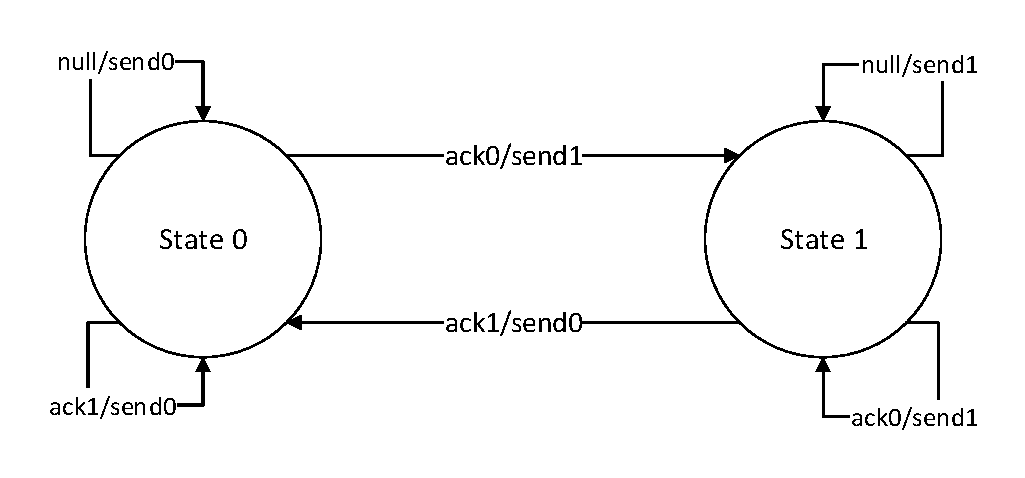
\includegraphics[width=1.0\linewidth]{figures/alternatingbit}
		\caption{Mealy machine representation of the alternating-bit protocol.}
	\end{subfigure}
	\begin{subfigure}{0.8\linewidth}
		\centering
		\begin{lstlisting}
			String sequence = 
				"null|send0|ack1|send0|ack0|send1"
				+ "|ack0null|send1|ack0ack0|send1|ack0ack1|send0"
				+ "|ack1null|send0|ack1ack0|send1|ack1ack1|send0"
				+ "|nullnull|send0|nullack0|send1|nullack1|send0"
				+ "|ack0nullnull|send1|ack0nullack0|send1|ack0nullack1|send0"
				+ "|ack0ack0null|send1|ack0ack0ack0|send1|ack0ack0ack1|send0"
				+ "|ack0ack1null|send0|ack0ack1ack0|send1|ack0ack1ack1|send0"
				+ "|ack1nullnull|send0|ack1nullack0|send1|ack1nullack1|send0"
				+ "|ack1ack0null|send1|ack1ack0ack0|send1|ack1ack0ack1|send0"
				+ "|ack1ack1null|send0|ack1ack1ack0|send1|ack1ack1ack1|send0"
				+ "|nullnullnull|send0|nullnullack0|send1|nullnullack1|send0"
				+ "|nullack0null|send1|nullack0ack0|send1|nullack0ack1|send0"
				+ "|nullack1null|send0|nullack1ack0|send1|nullack1ack1|send0";
		\end{lstlisting}
		\caption{}
	\end{subfigure}
	\caption{A Mealy machine \textbf{(a)}, with its input format \textbf{(b)} using the formalism described in Section \ref{item:stringsequencelearnable}s \emph{StringSequenceLearnable} item.}
	\label{fig:alternatingbit}
\end{figure}


\begin{lstlisting}[caption=Brute-force implementation of equivalence queries described in Section \ref{item:stringsequencelearnable}s \emph{StringSequenceAdapter} item using google guavas Sets.powerSet() function.,label=li:eqbruteforce,float,floatplacement=H]
@Override
public List<? extends I> equivalenceQuery(H hypothesis, Collection<? extends I> alphabet) {
	for(Set<I> s : com.google.common.collect.Sets.powerSet(new HashSet<I>(alphabet))) {
		if(!s.isEmpty()) {
			for(List<I> permutation : com.google.common.collect.Collections2.permutations(s)) {
				if(!hypothesis.query(permutation).equals(this.membershipQuery(permutation))) {
					O a = hypothesis.query(permutation);
					O b = this.membershipQuery(permutation);
					return permutation;
				}
			}
		}
	}
	return null;
}
\end{lstlisting}

\begin{lstlisting}[caption=The output MealyMachine after running the implemented TTT algorithm with the input seen in Listing \ref{li:4ixtext}.,label=li:xtextttt,float,floatplacement=H]
MealeyMachine{
	initialState State s0
	states {State s0,State s1,State s2,State s3,}
	transitions {
		Transition { input a output top sourceState s0 targetState s1},
		Transition { input b output top sourceState s0 targetState s0},
		Transition { input a output top sourceState s1 targetState s2},
		Transition { input b output top sourceState s1 targetState s1},
		Transition { input a output bot sourceState s2 targetState s3},
		Transition { input b output top sourceState s2 targetState s2},
		Transition { input a output top sourceState s3 targetState s0},
		Transition { input b output bot sourceState s3 targetState s3} }
}
\end{lstlisting}


\begin{lstlisting}[caption=The output MealyMachine after running the implemented DHC algorithm with the input seen in Listing \ref{li:4ixtext}.,label=li:xtextdhc,float,floatplacement=H]
MealeyMachine{
	initialState State state0
	states {State state0,State state1,State state2,State state3,}
	transitions {
		Transition { input a output top sourceState state0 targetState state1},
		Transition { input b output top sourceState state0 targetState state0},
		Transition { input a output top sourceState state1 targetState state2},
		Transition { input b output top sourceState state1 targetState state1},
		Transition { input a output bot sourceState state2 targetState state3},
		Transition { input b output top sourceState state2 targetState state2},
		Transition { input a output top sourceState state3 targetState state0},
		Transition { input b output bot sourceState state3 targetState state3} }
}
\end{lstlisting}

\begin{lstlisting}[caption=The output MealyMachine after running the implemented DHC algorithm with the input seen in Listing \ref{li:coffeemealy}.,label=li:coffeedhcret,float,floatplacement=H]
MealeyMachine{
	initialState State state0
	states {State state0,State state1,State state2,State state3,State state4,State state5,}
	transitions {
		Transition { input water output done sourceState state0 targetState state1},
		Transition { input pod output done sourceState state0 targetState state2},
		Transition { input button output none sourceState state0 targetState state3},
		Transition { input clean output done sourceState state0 targetState state0},
		Transition { input water output done sourceState state1 targetState state1},
		Transition { input pod output done sourceState state1 targetState state4},
		Transition { input button output none sourceState state1 targetState state3},
		Transition { input clean output done sourceState state1 targetState state0},
		Transition { input water output done sourceState state2 targetState state4},
		Transition { input pod output done sourceState state2 targetState state2},
		Transition { input button output none sourceState state2 targetState state3},
		Transition { input clean output done sourceState state2 targetState state0},
		Transition { input water output none sourceState state3 targetState state3},
		Transition { input pod output none sourceState state3 targetState state3},
		Transition { input button output none sourceState state3 targetState state3},
		Transition { input clean output none sourceState state3 targetState state3},
		Transition { input water output done sourceState state4 targetState state4},
		Transition { input pod output done sourceState state4 targetState state4},
		Transition { input button output coffee sourceState state4 targetState state5},
		Transition { input clean output done sourceState state4 targetState state0},
		Transition { input water output none sourceState state5 targetState state3},
		Transition { input pod output none sourceState state5 targetState state3},
		Transition { input button output none sourceState state5 targetState state3},
		Transition { input clean output done sourceState state5 targetState state0} }
}
\end{lstlisting}

\begin{lstlisting}[caption=The output MealyMachine after running the implemented DHC algorithm with the input seen in Listing \ref{li:coffeemealy}.,label=li:coffeetttret,float,floatplacement=H]
MealeyMachine{
	initialState State s0
	states {State s0,State s1,State s2,State s3,State s4,State s5,}
	transitions {
		Transition { input water output done sourceState s0 targetState s2},
		Transition { input pod output done sourceState s0 targetState s4},
		Transition { input button output none sourceState s0 targetState s1},
		Transition { input clean output done sourceState s0 targetState s0},
		Transition { input water output none sourceState s1 targetState s1},
		Transition { input pod output none sourceState s1 targetState s1},
		Transition { input button output none sourceState s1 targetState s1},
		Transition { input clean output none sourceState s1 targetState s1},
		Transition { input water output done sourceState s2 targetState s2},
		Transition { input pod output done sourceState s2 targetState s3},
		Transition { input button output none sourceState s2 targetState s1},
		Transition { input clean output done sourceState s2 targetState s0},
		Transition { input water output done sourceState s3 targetState s3},
		Transition { input pod output done sourceState s3 targetState s3},
		Transition { input button output coffee sourceState s3 targetState s5},
		Transition { input clean output done sourceState s3 targetState s0},
		Transition { input water output done sourceState s4 targetState s3},
		Transition { input pod output done sourceState s4 targetState s4},
		Transition { input button output none sourceState s4 targetState s1},
		Transition { input clean output done sourceState s4 targetState s0},
		Transition { input water output none sourceState s5 targetState s1},
		Transition { input pod output none sourceState s5 targetState s1},
		Transition { input button output none sourceState s5 targetState s1},
		Transition { input clean output done sourceState s5 targetState s0} }
}
\end{lstlisting}

%\label{page:last}
\end{document}
